\chapter{Uncertainty-Aware Data Flow Analysis to Identify Confidentiality Violations}%
\label{ch:confidentialityanalysis}%
 

In this chapter, we present the third Contribution \C{3}.
This contribution covers the last activity of the procedure shown in \autoref{sec:overview:procedure}, the confidentiality analysis with respect to uncertainty.
We discuss the representation of uncertainty as a first-class entity in data flow analysis and introduce four approaches for uncertainty-aware confidentiality analysis.

Software systems are becoming increasingly complex, e.g., in Industry 4.0 \cite{boltz_context-based_2020} or automotive systems \cite{acosta_uncertainty_2022}.
As stated previously, ensuring security-related quality properties like confidentiality becomes a major challenge.
Violations cannot only have legal consequences \cite{isaak_user_2018} but also affect user acceptance \cite{weisbaum_trust_2018}.
As proposed by \emph{Privacy by Design} \cite{schaar_privacy_2010}, confidentiality should be considered early to avoid costly repairs \cite{boehm_software_2001}.
This can also seen with the new \enquote{Insecure Design} category from the \ac{OWASP} Top 10 \cite{OWASPTop10} list, which contains the top 10 categories of security problems for web applications. 

This problem has been addressed with design time confidentiality analysis.
By analyzing data flows \cite{seifermann_detecting_2022} or potential attack paths \cite{walter_architectural_2022-1,walter_architecture-based_2023-1} in modeled software architectures, confidentiality requirements \cite{hahner_modeling_2021} can be evaluated early.
We discussed these approaches in previous chapters, especially in \autoref{ch:impactanalysis}.
There, we built on the transformation from the \acf{ADL} \acf{PCM} to \acfp{DFD} in order to propagate uncertainty regarding confidentiality.
This transformation originates from an architecture-based data flow analysis to identify confidentiality violations already at design time \cite{seifermann_data-driven_2019,seifermann_detecting_2022,seifermann_architectural_2022}.
Based on an architectural description of the software system, violations of provided confidentiality requirements \cite{hahner_modeling_2021} can be identified.
This involves the model-based propagation of characteristics within the software architecture, which describe the flowing data and its properties regarding confidentiality.
In sum, these approaches enable software architects to assess the confidentiality of software systems.

However, in early development and in complex systems of systems, uncertainty exists about the software architecture and its environment \cite{acosta_uncertainty_2022}.
Our running example from \autoref{ch:runningexample} shows multiple uncertainty sources, e.g., user input (\U{1}), data processing (\U{2}), or deployment (\U{3}).
When ignored, these uncertainties affect both the precision and comprehensiveness of the results of confidentiality analysis \cite{hahner_classification_2023,hahner_dealing_2021,hahner_architectural_2021}.
The lack of information reduces the quality of the model's representation of the software system. 
This results in less accurate or even wrong predictions, made on the basis of the model. 
Although uncertainty-aware analyses of software architectures exist \cite{esfahani_guidearch_2013}, they usually focus on other quality properties like performance \cite{sobhy_evaluation_2021}.

To address this limitation, we present multiple approaches to architectural confidentiality analysis under uncertainty.
We build on the findings about \acp{DFD} and uncertainty from the previous chapters to define data flow analyses that identify violations of confidentiality requirements with respect to uncertainty.
Taking known uncertainty into account helps in making more comprehensive statements about a software system's confidentiality.
The handling of uncertainty can either be included as part of the analysis in a white-box manner or delegated to an uncertainty-aware framework \cite{acosta_uncertainty_2022}.
Here, we keep the architectural abstraction to enable design time analysis.
Similarly to the previous chapter, we also propose automated analysis and tool-supported modeling as \enquote{detecting confidentiality issues manually is not feasible} \cite{seifermann_data-driven_2019}.

In sum, to define uncertainty-aware data flow analysis, advances both in modeling and analysis of confidentiality and uncertainty are required.
As proposed by \textcite{garlan_software_2010}, we thereby include uncertainty as a first-class concern in the system design.
We present two approaches for confidentiality analysis that are tailored to single uncertainty types, e.g., environmental, or structural uncertainty, as well as two uncertainty type-agnostic approaches.
We also discuss common challenges and solutions in representing uncertainty in data flow analysis.
We summarize this research concern of uncertainty-aware data flow analysis regarding confidentiality in the third research question:

\RQthree

The remainder of this chapter is structured as follows:
First, we discuss the problem statement.
We then introduce a framework for architectural data flow analysis.
This framework builds on the architecture-based data flow analysis of \textcite{seifermann_architectural_2022,seifermann_identifying_2021}, but extends and simplifies both the modeling and the analysis.
It lays the foundation for the further analysis approaches presented in this section.
Afterward, we discuss how to represent uncertainty in data flow analysis.
Depending on the approach and the use of existing information, different statements about confidentiality and uncertainty can be derived.
Building on this, we present two approaches for uncertainty type-specific data flow analysis.
The first uses fuzzy inference \cite{klir_fuzzy_1995} together with data flow analysis to consider environment uncertainty.
The second extends the architectural optimization approach PerOpteryx \cite{koziolek_peropteryx_2011,koziolek_automated_2011} to consider the relation of structural uncertainty and confidentiality.
Additionally, we present an approach to tracing uncertainty in data flow analysis and an uncertainty type-agnostic approach to data flow analysis.
Last, we discuss the complexity of the different uncertainty-aware data flow analysis approaches.
We close the chapter by presenting assumptions and limitations and giving a summary.

\ownpublications{
\fancycite{boltz_handling_2022},
\fancycite{walter_architectural_2022},
\fancycite{hahner_model-based_2023},\linebreak
\fancycite{boltz_extensible_2024}
}





\section{Problem Statement}%
\label{sec:confidentialityanalysis:problem}

We summarize the problems \textbf{P1} -- \textbf{P3} addressed by Contribution \C{3}.
Finding solutions to these problems helps to provide a comprehensive answer to \RQ{3}.

\paragraph{P1: Extending data flow analysis to represent uncertainty}\label{p:3:1}
To consider uncertainty in architectural data flow analysis, we first require an extensible framework for data flow analysis \cite{boltz_extensible_2024}.
This framework lays the foundations for any type of uncertainty-aware data flow analysis that goes beyond black-box approaches \cite{walter_architectural_2022}.
By black-box approaches, we mean approaches to confidentiality analysis that do not consider uncertainty as a first-class entity but encapsulate an existing analysis into an uncertainty-aware framework.
Additionally, we need to understand how uncertainty can be represented in confidentiality analysis \cite{hahner_model-based_2023}.
This requires relating previous findings on modeling and propagating uncertainty in architectural models to data flow analysis.
We stress that there is no single solution to this problem but various solutions that exhibit different benefits and drawbacks.
A common baseline is envisaged to understand their characteristics and applications.

\paragraph{P2: Data flow analysis tailored to specific uncertaint types}\label{p:3:2}
To better understand the relation of uncertainty and confidentiality on architectural abstraction, we first strive to define architecture-based data flow analysis tailored for specific uncertainty types.
Here, we focus on uncertainty types that are common in software architectures.
This includes structural uncertainty due to \acfp{ADD} \cite{walter_architectural_2022,jansen_software_2005} and also environmental uncertainty that can indirectly affect confidentiality, e.g., due to access control decisions under uncertainty \cite{boltz_handling_2022,bures_capturing_2020}.
Although such focused analysis approaches are unable to analyze all uncertainty types that can affect confidentiality, they still provide precise results regarding single uncertainty types, especially compared to uncertainty-unaware confidentially analysis \cite{seifermann_architectural_2022}.
Additionally, they present an important step towards uncertainty type-agnostic data flow analysis \cite{hahner_model-based_2023}.

\paragraph{P3: Uncertainty type-agnostic data flow analysis} \label{p:3:3}
Ultimately, a comprehensive approach is required to analyze all uncertainty types that are relevant regarding confidentiality.
Building on the findings from \PR{3}{1} and \PR{3}{2}, this approach shall be able to handle all uncertainty types described in the uncertainty classification, presented in \autoref{ch:classification}.
This uncertainty type-agnostic approach needs modeling support for expressing uncertainty in architectural models that goes beyond the annotation of uncertainty sources required for uncertainty impact analysis, discussed in \autoref{ch:impactanalysis}.
A common approach to expressing uncertainty in architectural models is modeling variation scenarios \cite{troya_uncertainty_2021,walter_architecture-based_2023}.
However, analyzing variations---and especially combinations of variations---can quickly jeopardize the scalability \cite{walter_context-based_2023,walter_architecture-based_2023-1}.
Building on previous findings regarding the \acf{UIP} in \acp{DFD} can reduce the analysis complexity.





\section{A Framework for Architectural Data Flow Analysis}%
\label{sec:confidentialityanalysis:framework}

In this section, we build on an approach for architecture-based data flow analysis \cite{seifermann_architectural_2016,seifermann_data-driven_2019,seifermann_detecting_2022,seifermann_unified_2021,seifermann_architectural_2022} to present our extensible framework for architectural data flow analysis \cite{boltz_extensible_2024}.
This lays the foundation for further analysis approaches---which are not limited to uncertainty only---and also addresses Problem \PR{3}{1}.

In general, there are two ways to approach uncertainty-aware analysis \cite{acosta_uncertainty_2022,perez-palacin_dealing_2014}.
We use the common differentiation between \emph{white-box} analysis and \emph{black-box} analysis composition \cite{taghavi_survey_2023,heinrich_composing_2021}.
A black-box approach extends an analysis without knowing about the implementation details of the analysis and only uses its interfaces.
A white-box approach can use the internal details and data structures for the composition.
Both approaches have benefits and drawbacks, e.g., regarding expressiveness and maintainability.
Regarding uncertainty, we favor white-box analysis approaches as they enable the representation of uncertainty as a first-class entity within the analysis \cite{garlan_software_2010}.
However, this does not imply that black-box approaches are not feasible \cite{walter_architectural_2022}.
To enable white-box analysis, we require an extensible and stable analysis framework.

Regarding the architectural data flow analysis, the original Prolog-based implementation of \textcite{seifermann_architectural_2022} was hard to maintain and had a high resource demand, which severely limits the applicability for large software systems.
Although the analysis already used a model of a \ac{DFD} \cite{demarco_structure_1979} as an intermediate representation, it did not continue to follow the idea of using \acp{DFD} as the primary analysis artifact. 
With appropriate tool support, \acp{DFD} represent a powerful and commonly used mechanism for threat analysis \cite{bernsmed_adopting_2022} that helps in correctly identifying security-related issues \cite{schneider_how_2024}.
Thus, we revisited all aspects of the analysis like the transformation of \ac{PCM} models to \acp{DFD}, and the label propagation, and also reimplemented the analysis from scratch \cite{schwickerath_tool-supported_2023}.
This results in a more scalable and also easier-to-extend analysis framework \cite{boltz_extensible_2024}.
Additionally, the focus on \acp{DFD} as the primary analysis artifact simplifies the connection to uncertainty, as discussed in \autoref{sec:classification:dfd}. 
We introduced some of the underlying concepts already in \autoref{ch:foundations}.
For the scope of this work, we summarize the internal data structures and the analysis procedure and refer to our publications for more details \cite{schwickerath_tool-supported_2023,boltz_extensible_2024,hahner_modeling_2021}.


\subsection{Representing Data Flows in Data Flow Analysis}

As discussed in \autoref{sec:classification:dfd}, \acp{DFD} can be represented as \acfp{DAG}.
Using a simple graph structure simplifies the reasoning and the automated analysis regarding confidentiality.
We support the transformation of \acp{DFD}, which are based on the unified modeling primitives \cite{seifermann_unified_2021}, and also of \ac{PCM} models \cite{reussner_modeling_2016} to \acp{DAG}.
The former enables the manual definition of \acp{DFD}, and the latter extends the integration of architectural models in the data flow analysis \cite{seifermann_data-driven_2019}.

To represent data flows and their relations in \acp{DAG}, we use the notion of a \acf{TFG}.
Flow graphs represent the flow from one source to one or multiple sinks \cite{knuth_art_1997}.
However, regarding confidentiality, we are more interested in the relations of data flows from multiple sources to a single sink.
An example is the joint flow of multiple sensitive data flows into a single sink, e.g., pseudonymized data flowing together with information about the relation of the data to its originating users, which could violate confidentiality.
We use these transposed semantics of a flow graph, thus creating \acp{TFG}.
Reasoning about multiple, smaller \acp{TFG} instead of one large \ac{DAG} provides further benefits.
It represents a divide and conquer approach, as the data flows represented by \acp{TFG} are independent and can thus be analyzed independently \cite{seifermann_architectural_2022}.
This simplifies the analysis and increases its scalability \cite{schwickerath_tool-supported_2023}.
It is also more intuitive because confidentiality analysis represents identifying critical data flows to a single destination, i.e., critical \acp{TFG}.

\begin{figure}
    \centering
    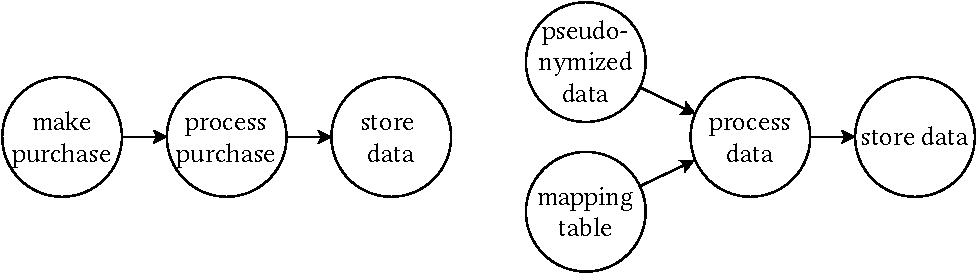
\includegraphics[width=\linewidth]{figures/chapter7/tfg.pdf}
    \caption{Two \acfp*{TFG} representing two independent data flows.}
    \label{fig:confidentialityanalysis:tfg}
\end{figure}

\autoref{fig:confidentialityanalysis:tfg} shows two \acp{TFG}.
The left \ac{TFG} represents a simple data flow from the running example presented in \autoref{ch:runningexample}.
The right \ac{TFG} represents the combination of data flows from two sources into a single sink, as discussed above with pseudonymized data.
We can see, that the data flows in \acp{TFG} inherit all properties from \ac{DAG}, i.e., being irreflexive, asymmetric, and transitive.
Additionally, starting from the single sink, all other vertices are reachable without cycles.
We can also see, that the partition in multiple, independent \acp{TFG} simplifies the reasoning.
In the example shown in \autoref{fig:confidentialityanalysis:tfg}, both \emph{store data} processes could be represented by the same call to a data base.
However, both data flows are independent, represent different data types and data processing, and also could cause different confidentiality violations.
For instance, storing data without encryption could violate the confidentiality in the \emph{store data} process in the left \ac{TFG}, while \emph{process data} could violate the confidentiality due to a broken pseudonymization in the right \ac{TFG}.

\finding{\acfp{TFG} show independent data flows of a \acf{DAG}.
Following the principle of divide and conquer, this simplifies reasoning about the variety of data flows in a system.}

To enable confidentiality analysis, we connect the concept of \acp{DAG} and \acp{TFG} to the unified modeling primitives \cite{seifermann_unified_2021}, introduced in \autoref{sec:foundations:dfd}.
Here, \emph{Nodes} and \emph{Flows} can be represented directly by vertices and edges, respectively.
Additionally, vertices can be annotated with \emph{Labels} to represent their characteristics regarding confidentiality, called \emph{node labels}.
Examples of such labels are the deployment location or the role of a user.
The \emph{Behavior} of a \emph{Node}, represented by one or multiple \emph{Assignments} can also be directly mapped to the vertices of a \ac{TFG}.
\emph{Assignments} can change the characteristics of flowing data, represented by \emph{data labels}.
For example, the behavior of the \emph{process purchase} vertex in \autoref{fig:confidentialityanalysis:tfg} could include setting an \emph{encrypted} label to represent the encryption of all data flows.
Last, \emph{Pins} are not directly represented in \acp{TFG} but influence their construction.
For instance, multiple \emph{Flows} out of a single \emph{Pin} represent alternatives that yield a \ac{TFG} for each alternative flow.
Again, for the scope of this work, we do not detail the transformation of \acp{DFD} to \acp{TFG}, but refer to the original publications \cite{seifermann_detecting_2022,boltz_extensible_2024}.

\begin{figure}
    \centering
    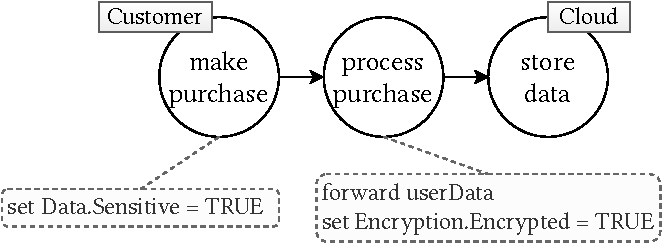
\includegraphics[width=0.7\linewidth]{figures/chapter7/annotatedtfg.pdf}
    \caption{A simple \acf*{TFG}, annotated with node labels and node behaviors.}
    \label{fig:confidentialityanalysis:annotatedtfg}
\end{figure}

\autoref{fig:confidentialityanalysis:annotatedtfg} shows the left \ac{TFG} from \autoref{fig:confidentialityanalysis:tfg}, annotated with node labels and behaviors, following the notation of the data flow analysis framework \cite{boltz_extensible_2024}.
The exemplary \emph{node labels} show which vertices represent functionality of the \emph{Customer}, or of components deployed in the \emph{Cloud}.
Note that there is no general rule on which characteristics can and should be represented by node labels---any information, that can be relevant for analyzing confidentiality, can be included within the model \cite{seifermann_architectural_2022}.
The exemplary node behaviors show how the \emph{data labels} can be altered.
First, the \emph{make purchase} vertex sets the label \emph{Data.Sensitive}.
Then, this label is forwarded in the \emph{process purchase} vertex, where also the label \emph{Encryption.Encrypted} is added.
Both labels flow to the \emph{store data} vertex.
In natural language, this simple \ac{TFG} represents sensitive user data that flows from a user into a database that is deployed in the cloud, while being encrypted first.
This notion simplifies reasoning about data flows regarding confidentiality and can also be applied to large \ac{DFD} with thousands of nodes \cite{schwickerath_tool-supported_2023}.

Confidentiality requirements can be formulated in the form of data flow constraints \cite{hahner_modeling_2021}.
These constraints restrict selected \emph{data labels} to never flow to selected \emph{node labels}.
In the example shown in \autoref{fig:confidentialityanalysis:annotatedtfg}, an exemplary data flow constraint could be that there shall not be a data flow of sensitive but unencrypted data to the cloud.
Due to the encryption in the vertex \emph{process purchase}, this data flow constraint is satisfied.
Thus, this constraint would not cause a confidentiality violation.
More complex constraints that consider the multiple flows and their properties are also possible \cite{hahner_modeling_2021,boltz_extensible_2024}.

\finding{\acfp{TFG} can be annotated with characteristics that represent system properties relevant for confidentiality analysis.
These characteristics comprise node labels, which are annotated to vertices, and data labels, which are altered by a node's behavior.
Confidentiality requirements can be represented as data flow constraints that compare node and data labels.}

Although the manual modeling of \acp{DAG} with confidentiality characteristics is possible \cite{boltz_extensible_2024}, we focus on the automated extraction of \acp{DAG} from \ac{PCM} models.
We introduced this extraction in \autoref{sec:impactanalysis:pcmpropagation}.
For instance, \emph{ExternalCallAction}, \emph{SetVariableAction}, and \emph{EntryLevelSystemCalls} are represented by \ac{DFD} nodes and thus also by \ac{TFG} vertices.
Additionally, we extract all confidentiality-related characteristics from the \ac{PCM} and represent them as node labels and data labels.

\begin{figure}
    \centering
    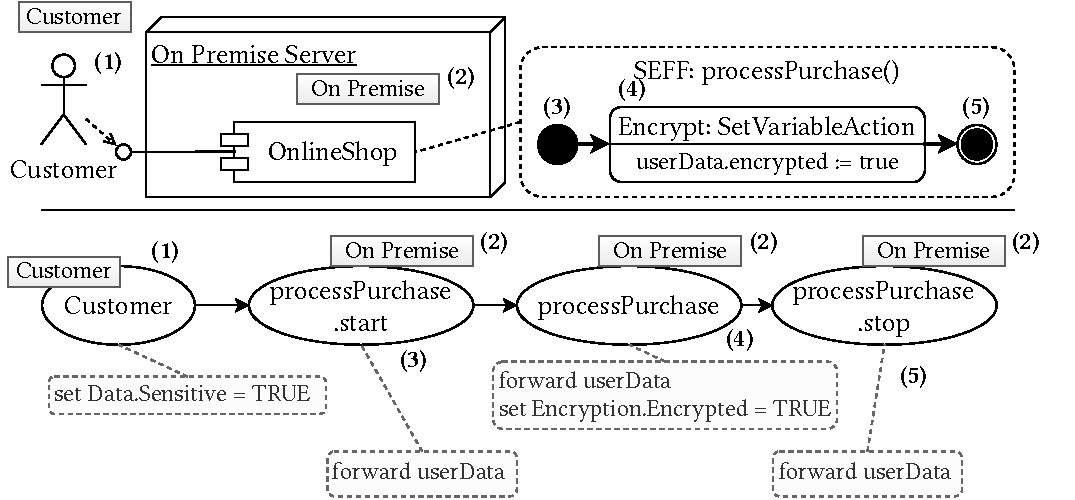
\includegraphics[width=\linewidth]{figures/chapter7/pcmextraction.pdf}
    \caption{Simplified \acf*{PCM} instance and the corresponding \acf*{TFG} with annotated node labels, data labels, and numbered transformation traces.}
    \label{fig:confidentialityanalysis:pcmextraction}
\end{figure}

\autoref{fig:confidentialityanalysis:pcmextraction} shows a simplified \ac{PCM} model based on the running example.
The model is annotated with confidentiality-related labels that represent characteristics of data storage like \emph{On Premise} and data processing like the encryption of \emph{userData} in the \emph{SetVariableAction}.
In the lower half, we show the extracted \ac{TFG}.
We annotate numbers to represent the transformation traces from the \ac{PCM} to the \ac{TFG}.
For every node, we perform a lookup of node labels, which can be annotated, e.g., to \emph{ResourceContainers}, or \emph{UsageScenarios}.
An exemplary lookup in the PCM model goes from the \emph{processPurchase} vertex to the \emph{Online Shop} component via the deployment to the \emph{On Premise Server} resource which is annotated with \emph{On Premise}.
Additionally, we convert the modeled system behavior to assignments representing the node's behavior, e.g., the encryption of \emph{userData}.
The default is the forwarding of labels, which represents the flow of data without further effects.
The transformation considers all information that is relevant for confidentiality analysis, e.g., data processing.
Other information is not transformed, e.g., components and servers do not cause additional elements in the \ac{TFG}.
This enables a system view from the perspective of the data.
We store all traces to the originating \ac{PCM} elements during the transformation.
This enables the evaluation of more advanced constraints in the data flow analysis.

In sum, \ac{TFG} represent a simple yet powerful way to reason about data flows, that can be extracted from \ac{PCM} models.
By adding node and data labels, they can represent the characteristics of the software system relevant for confidentiality analysis.
Data flow constraints can compare these labels to identify confidentiality violations.


\subsection{Label Propagation to Enable Scalable Confidentiality Analysis}

Annotated \acp{TFG} help to reason about data flows in software systems.
However, \acp{DFD} of realistic software systems contain several hundreds of nodes \cite{hahner_architecture-based_2023}.
\emph{Label propagation} has been proposed to automate the analysis, as manual analysis is not feasible \cite{seifermann_data-driven_2019}.
Put simply, label propagation propagates all data labels through all nodes of all \acp{TFG} with respect to the behavior of the nodes.

\begin{algorithm}
    \caption{Algorithm for vertex evaluation in \acfp*{TFG}}
    \label{alg:confidentialityanalysis:vertexevaluation}
    \begin{algorithmic}[1]
        \Procedure{\function{evaluateVertex}}{$\var{vertex}, \var{graph}$}
            \algindentskip
            \State $\var{vertex.nodelabels} \gets \function{evaluateNodeLabels}(\var{vertex})$ \Comment{Collect node labels} \label{alg:confidentialityanalysis:vertexevaluation:2}
            \State $\var{predecessors} \gets \function{getPredecessors}(\var{vertex})$
            \State $\var{vertex.datalabels} \gets \emptyset$
            \algblockskip

            \For{$\var{predecessor} \in \var{predecessors}$} \Comment{Collect data labels using recursion}
                \State $\var{vertex.datalabels} \gets \var{vertex.datalabels} \cup \function{evaluateVertex}(\var{predecessor}, \var{graph})$\label{alg:confidentialityanalysis:vertexevaluation:6}
            \EndFor
            \algblockskip

            \State $\var{result} \gets \function{evaluateNodeBehavior}(\var{vertex}, \var{vertex.datalabels})$ \label{alg:confidentialityanalysis:vertexevaluation:8}
            \State \Return{$\var{result}$}
            \algindentskip
        \EndProcedure   
    \end{algorithmic}
\end{algorithm}

\begin{algorithm}
    \caption{Algorithm for label propagation in \acfp*{TFG}}
    \label{alg:confidentialityanalysis:labelpropagation}
    \begin{algorithmic}[1]
        \Procedure{\function{labelPropagation}}{$\var{tfgs}$}
            \algindentskip

            \For{$\var{tfg} \in \var{tfgs}$} \Comment{Iterate over all independent TFGs}
                \State $\var{sink} \gets \function{getSink}(\var{tfg})$ \Comment{Start the evaluation at each sink}
                \State $\function{evaluateVertex}(\var{sink}, \var{tfg})$
            \EndFor
            \algblockskip

            \State \Return{$\var{tfgs}$}
            \algindentskip
        \EndProcedure   
    \end{algorithmic}
\end{algorithm}

\autoref{alg:confidentialityanalysis:vertexevaluation} shows the recursive algorithm of the vertex evaluation in label propagation, which resembles \ac{DFS}.
For each vertex, we first retrieve the vertex node labels in \autoref{alg:confidentialityanalysis:vertexevaluation:2}.
To simplify the algorithm, we denote the side effect of storing the labels in the vertex fields.
Afterward, we calculate the data labels that represent the output of the vertex and also store them in the corresponding vertex. 
This is achieved by recursively calling the calculation logic of all previous vertices and using the hereby calculated output labels as input, as shown in \autoref{alg:confidentialityanalysis:vertexevaluation:6}.
Before returning, we apply the behavior of the evaluated vertex to the input data labels in \autoref{alg:confidentialityanalysis:vertexevaluation:8}, e.g., altering the encryption label.
Note that we do not consider cycles in the propagation logic because \acp{TFG} represent \acp{DAG}.
Based on the evaluation of vertices, \autoref{alg:confidentialityanalysis:labelpropagation} shows the label propagation.
Here, we handle each \ac{TFG} separately as every \ac{TFG} represents independent data flows, and use the \emph{evaluateVertex} algorithm for the single sink of each \ac{TFG}.

\begin{figure}
    \centering
    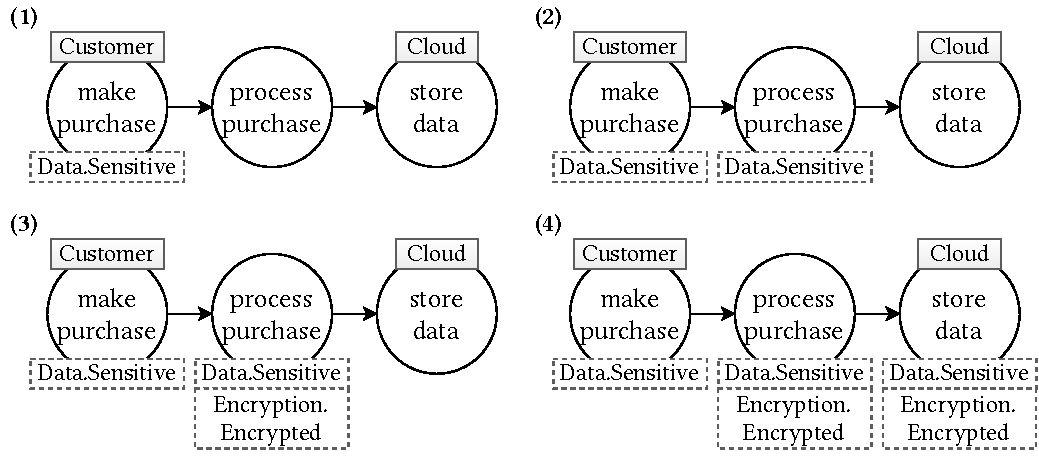
\includegraphics[width=\linewidth]{figures/chapter7/labelpropagation.pdf}
    \caption{Initial state, and intermediate and final results of the label propagation in a simple \acf*{TFG}. Node labels are highlighted gray, data labels have a dashed border.}
    \label{fig:confidentialityanalysis:labelpropagation}
\end{figure}

\autoref{fig:confidentialityanalysis:labelpropagation} shows four states of the label propagation in the simple \ac{TFG} introduced with \autoref{fig:confidentialityanalysis:annotatedtfg}.
First, we only display all node labels as these are not subject to label propagation but fixed, and also the label added in the \emph{make purchase} vertex.
This label is propagated to the \emph{process purchase} vertex in the second step.
By evaluating the behavior of this vertex, the label \emph{Encryption.Encrypted} is added in the third step.
In the fourth step, both labels are forwarded to the \emph{store data} vertex and the label propagation terminates.
After the label propagation, data flow constraints can compare node and data labels on each vertex without having to iterate over other vertices.
The resulting confidentiality analysis is scalable and has been evaluated on large \acp{DFD} with thousands of vertices \cite{schwickerath_tool-supported_2023}. 

\finding{Label propagation in \acfp{TFG} represents a simple and scalable way to automate data flow analysis regarding confidentiality.}





\section{Representing Uncertainty in Data Flow Analysis}%
\label{sec:confidentialityanalysis:representing}

The data flow analysis framework \cite{boltz_extensible_2024} presented in the previous section provides us with means for scalable confidentiality analysis and also with the notion of \acp{TFG} to reason about data flows.
The following discussion is based on this notion, and the differentiation between black-box and white-box analysis \cite{taghavi_survey_2023,heinrich_composing_2021}, presented in \autoref{sec:confidentialityanalysis:framework}.
We show different approaches to represent uncertainty in data flow analysis \cite{hahner_model-based_2023}.
These approaches differ in the use of data structures to analyze uncertainty and also in the use of information available for the analysis.
This addresses Problem \PR{3}{1}.

We addressed the representation of uncertainty in \ac{DFD}, in \autoref{sec:classification:dfd}, and in architectural models, in \autoref{sec:impactanalysis:representing}.
The former presented the distinction between \emph{primary} and \emph{secondary} uncertainty in \acp{DAG}, the latter related the five uncertainty types to elements of the unified modeling primitives \cite{seifermann_unified_2021} and to the \ac{PCM}.
We build on this to explain the representation of uncertainty in architecture-based data flow analysis.
As discussed previously, there are multiple approaches to data flow analysis under uncertainty which show different levels of uncertainty-awareness.
In the following, we discuss which information can be used for such analyses and present five levels of data flow analysis under uncertainty.


\subsection{Available Information in Uncertainty-Aware Data Flow Analysis}

\begin{table}
    \begin{tabularx}{\linewidth}{lX}
        \toprule
        Domain \, & Information categories \\
        \midrule
        Confidentiality & \mtl{
        \textbf{1.} Confidentiality violation occurrence, 
        \textbf{2.} Violated confidentiality\\requirements, 
        \textbf{3.} Location within the model,
        \textbf{4.} Analyzed data flows,\\ 
        \textbf{5.} State of data at the violation}
        \\
        \midrule
        Uncertainty & \mtl{
        \textbf{6.} Uncertainty source,
        \textbf{7.} Uncertainty properties and classification,\\
        \textbf{8.} Uncertainty impact within the model,
        \textbf{9.} Uncertainty interactions,\\
        \textbf{10.} Uncertainty mitigation}\\
        \bottomrule
    \end{tabularx}
    \caption{Available information categories for uncertainty-aware confidentiality analysis.}%
    \label{table:confidentialityanalysis:informationcategories}
\end{table}

\autoref{table:confidentialityanalysis:informationcategories} shows information categories regarding confidentiality and uncertainty.
The confidentiality information categories are derived from data flow-based analyses of architectural models \cite{seifermann_unified_2021}.
The categories include knowledge about the existence of confidentiality violations (\textbf{1.}) and the related violated requirements (\textbf{2.}).
We consider this to be the result of any usable analysis.
In the running example, the confidentiality requirements of storing personal data could be violated.
Additionally, such analyses can point to the location within the architectural model (\textbf{3.}) and the critical data flow (\textbf{4.}) where the violation occurred.
In the running example, the violating data flow could be from the \emph{Customer} to the \emph{Database Service}, where the violation happens.
Last, the state of the data causing the violation can be considered (\textbf{5.}).
This can be realized using labels like personal data, or deployment in the cloud.
The data flow analysis framework presented in \autoref{sec:confidentialityanalysis:framework} uses all five categories in the analysis and also when presenting identified confidentiality violations.
Nevertheless, analyses with a simplified interface are imaginable, e.g., black-box analyses only report the existence of violations.

The uncertainty information categories are derived from the uncertainty management in \acfp{SAS} \cite{hezavehi_uncertainty_2021} and \acfp{CPS} \cite{acosta_uncertainty_2022} and also based on the handling of uncertainty regarding confidentiality \cite{hahner_classification_2023}.
By investigating an uncertainty source (\textbf{6.}) in the model or its environment \cite{acosta_uncertainty_2022}, it can be described more precisely, e.g., based on a classification (\textbf{7.}), as discussed in \autoref{ch:classification}.
Also, the uncertainty's impact (\textbf{8.}) on the software architecture can be derived and expressed.
We discussed the distinction between uncertainty sources and their impact in \autoref{sec:classification:relation}.
In a software system with multiple uncertainty sources, potential uncertainty interactions are also important to consider (\textbf{9.}).
This is related to the \acf{UIP} and has been discussed with regard to \acp{DFD} in \autoref{sec:classification:dfd}.
Last, by analyzing the architectural model, mitigation techniques (\textbf{10.}) can be chosen already at design time \cite{hezavehi_uncertainty_2021}.
In our running example, we identified four uncertainty sources (\U{1} -- \U{4}), which were also classified.
We analyzed the potential impact of these uncertainties using uncertainty impact analysis in \autoref{ch:impactanalysis}.
For instance, uncertainty \U{4} causes a broad impact in the \emph{Database Service}.
We also have means to represent simple uncertainty interactions, e.g., between secondary and primary uncertainty sources in \acp{DAG}, see \autoref{sec:classification:dfd}.
For example, we identified an uncertainty interaction between the deployment in Uncertainty \U{3} and the provider trustworthiness in Uncertainty \U{4}.
Last, design time approaches can also support the tool-supported mitigation uncertainty that causes confidentiality violations.
We consider this to be out of scope for this work as we focus on the uncertainty-aware analysis as a required prerequisite for mitigation \cite{weyns_introduction_2020}.


\subsection{Levels of Uncertainty-Awareness in Data Flow Analysis}

Based on these information categories (\textbf{1.} -- \textbf{10.}), we define five levels (\level{0} -- \level{4}) of data flow analyses under uncertainty.
Regarding model-based confidentiality analysis, showing violations (\textbf{1.}) with the related reason (\textbf{2.}) to software architects is considered to be the minimum viable information \cite{hahner_modeling_2021}.
The analysis results become more expressive by also showing the location (\textbf{3.}), analyzed data flows (\textbf{4.}) and the state of the data (\textbf{5.}).


\paragraph{L0: No uncertainty-awareness}\label{awarenesslevel:0}
Data flow analyses that provide neither modeling nor analysis support for uncertainty show \emph{no uncertainty-awareness}.
This affects the precision and comprehensiveness \cite{hahner_architectural_2021} of confidentiality violations as the models and the analysis fall short of representing the real world, as discussed in the introduction of this chapter.
The lack of awareness becomes visible in over-estimations and also in missing violations \cite{seifermann_architectural_2022}.
In our running example, a confidentiality analysis that ignores uncertainty would miss all violations due to the identified uncertainty sources.
This level represents the state of the art before our endeavors \cite{seifermann_architectural_2022,hahner_dealing_2021,seifermann_detecting_2022}.
Note that this does not mean that such analyses cannot be extended to consider uncertainty \cite{hahner_dealing_2021}.


\paragraph{L1: Naive approach to uncertainty-awareness}\label{awarenesslevel:1}
The \emph{naive approach} to handling uncertainty is to directly model its impacts (\textbf{8.}).
This means manually altering models to respect the change caused by uncertainty.
In our running example, we can model different variants, e.g., with the deployment on-premise or in the cloud.
The analysis rejects the software architecture if there exist confidentiality violations in at least one variant.
By directly representing the uncertain effect within the model, we lose all information about the source (\textbf{6.} and \textbf{7.}).
Especially when considering multiple uncertainty impacts, all variant combinations and interactions (\textbf{9.}) have to be manually modeled, which requires extensive manual effort. 
Additionally, changes to the model have to be done in all variants.
While this yields more comprehensive results, it still highly lacks precision \cite{bitschi_uncertainty-aware_2022} and requires an unreasonably high manual effort.


\paragraph{L2: Scenario-awareness}\label{awarenesslevel:2}
\emph{Scenario-aware} analyses build on the idea of representing uncertainty sources (\textbf{6.}) as model variations separate from the modeled software architecture.
Here, variability models, model variations, or partial models represent common ways of expressing the potential outcomes of uncertainty \cite{troya_uncertainty_2021}.
We also included this level of information in our classification (\textbf{7.}).
The option \emph{Scenario Uncertainty} in the category \emph{Type} expresses a state of knowledge where the effects of an uncertainty source can be described using scenarios.
As classified in \autoref{sec:classification:runningexample}, all uncertainty sources are describable using scenarios in our running example.
The main difference to the \emph{naive approach} (\level{1}) is the automated application of these variations to the architectural model.
This approach greatly reduces the manual modeling effort, as software architects only have to specify the point of variation and do not realize the variation and thus the impact of the uncertainty (\textbf{8.}) itself.
The analysis rejects only such architecture variants that violate confidentiality, without considering the location (\textbf{3.}), data flows (\textbf{4.}) or the state of the data (\textbf{5.}).
Realized as a black-box analysis extension, this lacks precision because it only considers the existence of violations (\textbf{1.}) of requirements (\textbf{2.}) in selected scenarios.
Last, while the manual effort is reduced, the complexity of calculating variations of variations can quickly lead to a combinatorial explosion, as discussed in the context of design space exploration \cite{koziolek_automated_2011}.


\paragraph{L3: Graph-awareness}\label{awarenesslevel:3}
To overcome the limitations regarding scalability and expressiveness of the results, \emph{graph-aware} analyses can be used.
Realized as white-box extension \cite{boltz_architectural_2021,bitschi_uncertainty-aware_2022,boltz_handling_2022,hahner_architecture-based_2023} of a data flow analysis, this enables the connection of uncertainty sources (\textbf{6.}) to analyzed data flows (\textbf{4.}).
This is the first level that is able to represent uncertainty as a first-class concern, both within the architectural model and \acp{DFD}.
It builds on the idea of representing uncertainty as a set of scenarios, introduced with the \emph{scenario-aware} approach (\level{2}).
However, by relating the variation directly to the analyzed data flows, a higher expressiveness can be reached.
\emph{Graph-aware} analyses thus cover all five confidentiality related categories (\textbf{1.} -- \textbf{5.}) and are able to represent Uncertainty sources (\textbf{6.}), their properties (\textbf{7.}), and their impact (\textbf{8.}) directly within the model.
Additionally, they can achieve higher scalability as uncertainty sources in different data flows can be analyzed independently, which partially addresses the combinatorial explosion.
Put simply, in a real-world software system with many independent data flows, the effects of uncertainties can be separate.
To leverage this, the analysis requires awareness about the analyzed graph, which represents the main difference to the \emph{scenario-aware} approach (\level{2}).
In our running example, the \emph{scenario-aware} approach can only try out all variations, while the \emph{graph-aware} approach can use the information of the different data flows from the \emph{Customer}.
However, this does not lead to more accurate results---both approaches differ in expressiveness and scalability.
Note that we renamed \enquote{data flow-awareness} to \enquote{graph-awareness} compared to the original publication \cite{hahner_model-based_2023} to increase clarity\footnote{Like an uncertainty-aware uncertainty analysis, a data flow-aware data flow analysis does not make too much sense. However, I am not so sure about the former---what about antifragility?}.


\paragraph{L4: Impact-awareness}\label{awarenesslevel:4}
The \emph{graph-aware} analysis (\level{3}) is able to consider the effect of single uncertainty sources, both within the architectural model and \acp{DFD}.
However, the impact of uncertainties can also affect other uncertainties, i.e., uncertainty interaction.
This becomes visible in uncertainty-aware data flow analysis when an uncertainty alters a data flow that contains another uncertainty.
In our running example, such an interaction happens with Uncertainty \U{3} about the deployment and Uncertainty \U{4} about the provider's trustworthiness.
The former can impact the data flow so that it does not flow to a location that is affected by the latter, as shown in \autoref{fig:classification:dag}.
By understanding such interactions and the transitive effects of propagating uncertainty, and by incrementally analyzing data flows, \emph{impact-awareness} can be reached.
This level builds on the findings of \emph{scenario-aware} (\level{2}) and \emph{graph-aware} (\level{3}) approaches and thus yields analysis results with the same accuracy regarding confidentiality violations.
However, by also considering uncertainty interactions (\textbf{9.}), a higher expressiveness and scalability can be reached.


These five levels (\level{0} -- \level{4}) of uncertainty-aware data flow analysis provide the terminology to present the different research approaches hereafter.
Although the terminology is related to orders of ignorance \cite{armour_five_2000} or the levels of uncertainty \cite{bures_capturing_2020}, there exists no direct mapping, as we only focus on already identified uncertainty sources, see \autoref{ch:classification}.
Note that these levels do not represent a comprehensive list but only a classification for the scope of this work.
Further classes are imaginable, e.g., regarding the mitigation (\textbf{10.}), or by using advanced algorithms for analyzing uncertainty impacts and confidentiality violations.

Other classifications of uncertainty-aware data flow analyses are useful in addition to these levels.
Regarding the wide variety of uncertainty sources, some analyses might not cover all types of uncertainty \cite{troya_uncertainty_2021,PSUM}.
\textcite{troya_uncertainty_2021} conduced a \acf{SLR} with 123 papers and found that the majority of approaches only consider less than three types of uncertainty, e.g., behavior uncertainty combined with design uncertainty or belief uncertainty combined with measurement uncertainty.
Here, we build on the five uncertainty types of the category \emph{Architectural Element Type} of our classification, introduced in \autoref{sec:classification:classification}.
We call an uncertainty-aware data flow analysis to be \emph{type-specific} if it supports a subset of these uncertainty types.
Uncertainty \emph{type-agnostic} approaches support all five uncertainty types.

\finding{Uncertainty-aware data flow analysis approaches can be classified depending on the supported uncertainty types and the utilization of available information within the analysis.
This enables the classification of approaches that differ in accuracy, expressiveness, and scalability.}


\subsection{Examples for Uncertainty-Aware Data Flow Analysis}

\begin{table}
    \begin{tabularx}{\linewidth}{llX}
        \toprule
        \multicolumn{2}{l}{Uncertainty source} & Uncertainty scenarios \\
        \midrule
        \U{1} & User input & Valid input \,/\, Erroneous input \,/\, Malicious input \\
        \U{2} & Data processing & None \,/\, Encryption \,/\, Validation \,/\, Both \\
        \U{3} & Component deployment & On premise \,/\, Cloud service \\
        \U{4} & Provider trustworthiness & Trustworthy \,/\, Suspicious \\
        \bottomrule
    \end{tabularx}
    \caption{Uncertainty scenarios of all uncertainty sources of the running example.}%
    \label{table:confidentialityanalysis:scenarios}
\end{table}

We illustrate the different levels (\level{0} -- \level{4}) and types of uncertainty-aware analysis using our running example.
As discussed previously, all four uncertainty sources (\U{1} -- \U{4}) represent \emph{Scenario} uncertainty.
Based on the findings of \textcite{troya_uncertainty_2021}, we can thus describe the variation scenarios of all four uncertainty sources.
\autoref{table:confidentialityanalysis:scenarios} shows the possible scenarios for each uncertainty source that has been introduced in \autoref{ch:runningexample}.

A data flow analysis that lacks uncertainty-awareness (\level{0}) is not able to consider these uncertainty sources.
Speaking in terms of variations, these analyses select one scenario of each uncertainty, i.e., the architectural model without modification.
Only if this default scenario violates confidentiality, the violation is identified.
The \emph{naive} approach (\level{1}) to uncertainty-aware analysis is to manually model all combinations of all scenarios.
As this approach must assume the dependence of all uncertainty sources and their scenarios, we use the Cartesian product \cite{de_finetti_theory_2017}.
Thus, software architects have to manually model $3 \cdot 4 \cdot 2 \cdot 2 = 48$ software architectures in the running example, which is not feasible.

Using variation models in \emph{scenario-aware} analysis (\level{2}), software architects only model the variation points, i.e., all $3 + 4 + 2 + 2 = 11$ scenarios of the running example.
The variation creation can be automatized \cite{walter_architecture-based_2023}, which reduces the manual modeling effort, i.e., $11 < 48$.
However, the assumption on the dependence of all uncertainty sources remains and thus, all resulting $48$ variants have to be analyzed.
With larger amounts of uncertainty sources or scenarios, this can quickly lead to the already discussed combinatorial explosion \cite{koziolek_automated_2011}.

The \emph{graph-aware} approach (\level{3}) addresses this issue.
As discussed with uncertainty propagation in \ac{DFD} in \autoref{sec:impactanalysis:dfdpropagation}, uncertainty sources can be considered independently in all independent data flows.
This reduces the number of variants that have to be analyzed in all non-trivial software systems, i.e., in software systems with more than a single data flow.
Our running example comprises three independent data flows: Retrieving the support contact, querying items, and making purchases, see \autoref{fig:runningexample:dfd}.
Using the \ac{DFD} as a data structure for the analysis, the \emph{graph-aware} approach yields more comprehensive results.
In our running example, we can see that the data flow representing the support contact retrieval is neither affected by uncertainty nor violates confidentiality.

Last, the \emph{impact-aware} approach (\level{4}) builds on this and also considers uncertainty interactions.
We discussed this with the interaction of the uncertainties \U{3} and \U{4} in \autoref{sec:classification:dfd}.
Note that we do not classify the uncertainty impact analysis presented in \autoref{ch:impactanalysis} as it does not represent a confidentiality analysis.
However, this analysis could be considered as type-agnostic and graph-aware, as all five uncertainty types can be propagated on the \ac{DFD}.
This analysis does not reach \emph{impact-awareness} because the effect of changes to the software architecture is ignored and overestimated.

\begin{table}
    \begin{tabularx}{\linewidth}{llXX}
        \toprule
        \multicolumn{2}{l}{Level of awareness} & Uncertainty type-specific & Uncertainty type-agnostic \\
        \midrule
        \level{0} & None & \multicolumn{2}{l}{Uncertainty-unaware data flow analysis \cite{seifermann_detecting_2022,seifermann_architectural_2022,boltz_extensible_2024}} \\
        \midrule
        \level{1} & Naive & - & - \\
        \level{2} & Scenario-aware & Approach for structural uncertainty, \autoref{sec:confidentialityanalysis:structural} & - \\
        \level{3} & Graph-aware & Approach for environmental uncertainty, \autoref{sec:confidentialityanalysis:environmental} & Approach for tracing uncertainty, \autoref{sec:confidentialityanalysis:tracing} \\
        \level{4} & Impact-aware & - & Approach for impact-aware analysis, \autoref{sec:confidentialityanalysis:abunai} \\
        \bottomrule
    \end{tabularx}
    \caption{Awareness levels and type specificity of uncertainty-aware data flow analysis approaches.}%
    \label{table:confidentialityanalysis:awareness}
\end{table}

In the remainder of this chapter, we present four approaches to uncertainty-aware data flow analysis.
\autoref{table:confidentialityanalysis:awareness} classifies these approaches according to the five levels (\level{0} -- \level{4}) and with regard to the type specificity.
We also add the \emph{uncertainty-unaware} approach of architecture-based data flow analysis for reference purposes.

The data flow analysis framework \cite{boltz_extensible_2024} without explicit support for modeling or analyzing uncertainty as presented in \autoref{sec:confidentialityanalysis:framework} represents Level \level{0}.
We do not distinguish between the type specificity as the analysis does support no uncertainty at all.
We also do not present naive approaches (\level{1}) in this thesis, as they do not represent a noteworthy improvement on the state of the art.
The first approach discussed in this thesis is the \emph{scenario-aware} analysis (\level{2}) of structural uncertainty, e.g., regarding uncertain component deployment.
Due to the previously discussed limitations of scenario awareness, we continue with an approach for environmental uncertainty that is \emph{graph-aware} (\level{3}).
Afterward, we present the first uncertainty type-agnostic approach for data flow analysis.
This approach covers all five uncertainty types and traces confidentiality violations to variations caused by uncertainty sources.
Last, we further enhance this concept and present an uncertainty \emph{impact-aware} approach (\level{4}) for data flow analysis regarding confidentiality.
Generally speaking, a higher level and being type-agnostic is superior.





\section{Uncertainty Type-Specific Data Flow Analysis}%
\label{sec:confidentialityanalysis:typespecifc}

In this section, we present the first two approaches for uncertainty-aware data flow analysis.
The first approach is \emph{scenario-aware} (\level{2}) and considers structural uncertainty within the software architecture.
The second approach is \emph{graph-aware} (\level{3}) and deals with environmental uncertainty concerning user privileges in access control.
Both approaches are \emph{type-specific} as they are tailored to one uncertainty type.
This addresses Problem \PR{3}{2}.


\subsection{Data Flow Analysis Under Structural Uncertainty}%
\label{sec:confidentialityanalysis:structural}

As the name suggests, structural uncertainty affects the structure of the software architecture.
Examples are \acfp{ADD} regarding components or their deployment.
As this represents uncertainty in the software design \cite{mcconnell_software_1998}, it is best represented using variation points \cite{troya_uncertainty_2021}.
Regarding the variation creation, there already exist approaches such as design space exploration \cite{sobhy_evaluation_2021}.
For this analysis approach, we use the architectural optimization approach PerOpteryx \cite{koziolek_automated_2011,koziolek_performance_2010,koziolek_peropteryx_2011,martens_automatically_2010} and combine it with data flow analysis \cite{seifermann_detecting_2022}.
Software architects first model different design decisions. 
These design decisions are then used to automatically create different architecture variations, which are analyzed for confidentiality.
Since we reuse PerOpteryx for the design space exploration, this approach can consider additional quality attributes, such as performance, or costs, and calculate the Pareto optimal candidate.
This optimization enables software architects to make informed trade-off decisions between quality metrics.

PerOpteryx \cite{koziolek_peropteryx_2011,koziolek_automated_2011} is a design space exploration and optimization approach for the \ac{PCM}. 
It uses evolutionary search algorithms and calculates the Pareto optimal architectural variation. 
The different variation points of the architecture are specified in the design decision model. 
Here, software architects can define which entities in the software architecture can be configured. 
For instance, in our running example, a design decision is the deployment of the \emph{Database Service} component to the \emph{On Premise Server} or to the \emph{Cloud Service}.
Due to the relation of \acp{ADD} and uncertainty, explained in \autoref{sec:classification:relation}, we can use this model to express structural uncertainty sources and their scenarios.
The different quality attributes are defined as quality dimensions.
Each generated architectural variation that is evaluated for quality attributes is called a candidate. 
Besides the optimal candidates, PerOpteryx also yields all the investigated candidates.
There exist various quality dimensions, such as costs or performance. 
However, there is no quality dimension for confidentiality, which is required for the connection to the data flow analysis. 
While PerOpteryx already contains a security dimension \cite{busch_modelling_2016}, we decide against it since we want to explicitly target confidentiality. 
The existing security dimension is focused more on the costs of introducing security measures and the costs of failure.

\begin{figure}
    \centering
    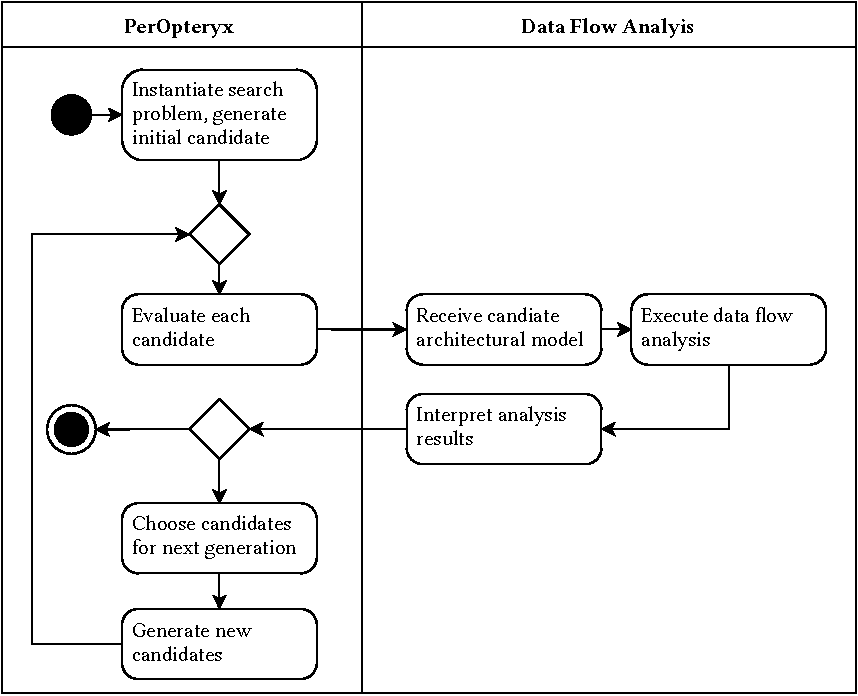
\includegraphics[width=\textwidth]{figures/chapter7/peropteryx.pdf}
    \caption{Activity diagram showing the interplay of PerOpteryx and the data flow analysis using swimlanes.}
    \label{fig:confidentialityanalysis:peropteryx}
\end{figure}

We add a new confidentiality violation to PerOpteryx that is modeled as real values where decreasing values are better solutions \cite{liu_design_2021}.
We map these to a binary classification for the confidentiality analysis results.
For each quality dimension, PerOpteryx defines handlers, which can analyze a model for the given quality dimension. 
Therefore, we define a new confidentiality handler for the confidentiality domain, which acts as an adapter between PerOpteryx and the data flow analysis.
This handler forwards the current architecture candidate models to the data flow analysis and interprets the analysis result.
The interpretation of confidentiality violations is binary with the classes \emph{confidentiality ensured} and \emph{confidentiality violated}. 
Our adapter transforms \emph{confidentiality ensured} to -1 and \emph{confidentiality violated} to 1.
This binary interpretation is required as there is currently no meaningful way of further quantifying the results of the data flow analysis \cite{walter_architectural_2022}.
The results enable the PerOpteryx optimization to rank confidential candidates higher than non-confidential ones.
After the execution of PerOpteryx, software architects get a result with all tested variations and the Pareto optimal version.
\autoref{fig:confidentialityanalysis:peropteryx} shows this procedure of PerOpteryx \cite{koziolek_peropteryx_2011} using the data flow analysis.
For the sake of simplicity, we only depict a single quality dimension, i.e., confidentiality.
Other quality dimensions can be represented by additional swimlanes that are called during the candidate evaluation.

In our running example, only Uncertainty \U{3} about the deployment represents structural uncertainty.
This uncertainty can be modeled as \ac{ADD} in the design decision model.
PerOpteryx then creates all variations, i.e., the deployment on the \emph{On Premise Server} and on the \emph{Cloud Service}.
Both candidates are forwarded to the data flow analysis.
The former ensures confidentiality while the latter causes a confidentiality violation and thus returns the value 1.
Last, the deployment \emph{on premise} is returned as the optimal version.

There are three disadvantages and two advantages of this approach.
First, being type-specific to structural uncertainty limits the applicability to other uncertainty types that can affect confidentiality.
Second, the black-box coupling of PerOpteryx with the data flow analysis only shows the existence of violations but no further information, e.g., on the location, or affected data flows, which impedes the interpretation by software architects.
Third, confidentiality violations have no continuous occurrence, i.e., small changes to the software architecture can have a large impact.
This is a known limitation of PerOpteryx and is described as a rugged search landscape with non-continuous jumps \cite{koziolek_automated_2011}.
In the worst case, this can cause PerOpteryx to test out all possible variations, i.e., the Cartesian product, which resembles a brute-force approach.
Nevertheless, this coupling is superior to the \emph{naive} approach (\level{1}) as it notably reduces the modeling effort.
Additionally, combining confidentiality analysis with the optimization of other quality attributes represents a more realistic application scenario, where informed trade-off decisions are made by software architects.
No other approach presented in this thesis provides such functionality without requiring the combination with other architecture evaluation approaches \cite{sobhy_evaluation_2021}.

\finding{On the one hand, the black-box coupling of data flow analysis with architectural optimization is complicated by the non-continuous occurrence of confidentiality violations, which increases the complexity of the optimization problem.
On the other hand, extending an existing software architecture optimization approach simplifies the joint evaluation of multiple quality attributes.}

\begin{algorithm}
    \caption{Algorithm for scenario-aware data flow analysis under uncertainty}
    \label{alg:confidentialityanalysis:scenarioaware}
    \begin{algorithmic}[1]
        \Procedure{\function{analyzeScenarioAware}}{$\var{model}, \var{constraint}, \var{uncertainties}$}
            \algindentskip
            \State $\var{violations} \gets \emptyset$
            \State $\var{variations} \gets \function{generateAllVariations}(\var{model}, \var{uncertainties})$
            \algblockskip

            \For{$\var{variation} \in \var{variations}$} \Comment{Analyze all possible variations}
                \State $\var{violations} \gets \var{violations} \cup \function{analyze}(\var{variation}, \var{constraint})$ 
            \EndFor
            \algblockskip

            \State \Return{$\var{violations}$}
            \algindentskip
        \EndProcedure   
    \end{algorithmic}
\end{algorithm}

To conclude, we present a more general approach to \emph{scenario-aware} data flow analysis under uncertainty.
Put simply, \emph{scenario-awareness} (\level{2}) is generating all possible variations of the architectural model and then analyzing them to identify confidentiality violations \cite{walter_architecture-based_2023}.
This is shown in \autoref{alg:confidentialityanalysis:scenarioaware}.
However, such analyses are prone to the combinatorial explosion of uncertainty sources and their scenarios.
Additionally, the analysis results are hard to interpret without further processing.
For instance, in our running example, software architects would have to interpret the confidentiality violations of 48 architectural models to asses four uncertainty sources.
We posit that \emph{scenario-aware} analysis should only be used in specific cases, e.g., combined with design space exploration. 


\subsection{Data Flow Analysis Under Environmental Uncertainty}%
\label{sec:confidentialityanalysis:environmental}

Environmental uncertainty arises from the system context, e.g., in the system usage, or its resource environment.
Here, sensors are especially often referred to as uncertainty source \cite{camara_addressing_2022,camara_uncertainty_2024,perez-palacin_uncertainties_2014,camara_software_2020,weyns_introduction_2020}.
Examples are sensor failure, sensor noise, or sensor inaccuracy \cite{hahner_arcn_2024}.
We discussed the relation of such uncertainty and confidentiality in \autoref{ch:classification}, where we classified such uncertainty as \emph{environment} or \emph{input} uncertainty.
A particular challenge is the relation of environmental uncertainty and access control \cite{bures_capturing_2020,heinrich_dynamic_2023}.
Broken access control can lead to severe confidentiality violations and is listed as the TOP 1 entry in the \ac{OWASP} Top 10 \cite{OWASPTop10}.
To address this, we present our second approach to uncertainty-aware data flow analysis: A \emph{graph-aware} analysis (\level{3}) of environmental uncertainty.
The following description is based on our publication about this approach \cite{boltz_handling_2022}.

A common measure to ensure confidentiality are access control mechanisms that authorize access or processing of data. 
Depending on the underlying access control model, various sources of information are used to determine whether access is granted. 
Services use different sources, e.g., sensors, to acquire information. 
Services process the information and provide a resulting access control attribute, e.g., a role or a location, that can be used by the access control system. 
However, these services introduce a degree of uncertainty to the access control system. 
This uncertainty results from influencing factors of the environment when acquiring the information. 
The influence of the factors on the access control system can result in reduced validity of statements about confidentiality. 
Depending on the system design, software architects or security experts might already be able to identify potential influencing factors. 
For example, the ability of a GPS service to provide an accurate position is highly dependent on its surroundings, like buildings. 

We extend our running example presented in \autoref{ch:runningexample} to illustrate this challenge.
We add an \emph{Admin} user who can directly access the \emph{Database Service} for maintenance \cite{walter_context-based_2023}.
To enhance security, access to the database is only permitted if the accessing actor is located inside of the office. 
The location of each actor is monitored using a GPS location service.
Here, we can choose a high-sensitivity GPS sensor, short \emph{HSGPS}, or the normal GPS sensor in the actor's mobile phone.
For this example, we focus on the differences between running the two types of GPS sensors indoors \cite{kjaergaard_indoor_2010}, where the sensor quality can degrade.
Once the actor enters the building, the signal attenuation increases which results in a reduced signal-to-noise ratio.
A reduced signal-to-noise ratio increases the time needed to acquire satellite data and calculate a position, and the amount of positioning errors \cite{kjaergaard_indoor_2010}. 
While the HSGPS sensors are powerful enough to provide accurate positioning, the accuracy of the embedded GPS sensor of the mobile phone suffers when used inside, which leads to uncertainty regarding the actual position. 
This reduced accuracy introduces uncertainty about the position \cite{camara_software_2020}. 
When this information is used within access control, it could lead to the wrong classification of the \emph{Admin} or other actors in the building.

To address such uncertainty, we present an approach for handling known, environmental uncertainty in access control during design time.
To this end, we enable the explicit representation of the known uncertainty and integrate the additional knowledge into an analysis. 
We propose a notion of \emph{confidence} in the validity of access control attributes, based on three types of influencing factors of the system environment.
We then show an access control analysis that integrates \emph{confidence} into our data flow analysis framework, presented in \autoref{sec:confidentialityanalysis:framework}. 
We propose the use of \acfp{FIS} \cite{klir_fuzzy_1995} to combine influencing factors to a resulting confidence value.

\begin{figure}
    \centering
    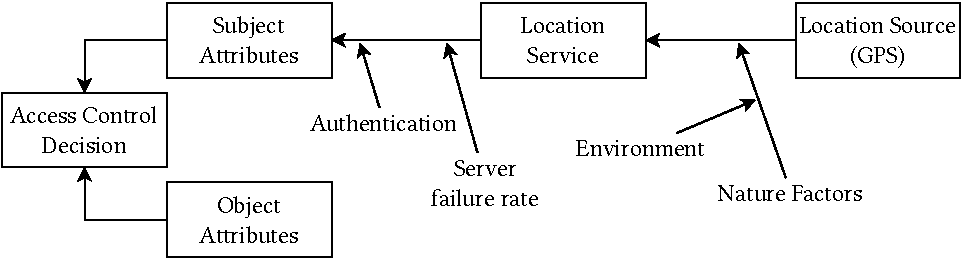
\includegraphics[width=\linewidth]{figures/chapter7/trustchain.pdf}
    \caption{A simplified trust chain that incorporates types of factors of the GPS location example.}
    \label{fig:confidentialityanalysis:trustchain}
\end{figure}

\textcite{hu_guide_2014} provide a definition and considerations regarding \acf{ABAC}. 
They describe a trust chain, concerning the attributes used to make access control decisions. 
Trust chains help determine the ownership of information and services, as well as requirements for technical solutions to establish valid trust relationships. 
The predicate of a trust relationship revolves around the idea that the access control system can trust the validity or correctness of the information, supplied by the owner, e.g., an authorization service. 
Depending on the access control model, many trust relationships are required to achieve a properly working access control system.
\autoref{fig:confidentialityanalysis:trustchain} shows a trust chain of a location attribute. 
The \emph{subject attributes} have a trust relationship with the \emph{location service}, which in turn has a trust relationship with the \emph{location source}. 
As indicated by the additional arrows, the trust relationships are impacted by influences of the environment of the system.

\textcite{ardagna_supporting_2006} define a confidence value that combines the service used for location determination and environmental conditions. Similar to the trust of \textcite{hu_guide_2014}, confidence describes the certainty that a location is valid, which is dependent on the environment.
Based on the work of \textcite{hengartner_distributed_2007} we can identify three environmental factors that influence the uncertainty in access control. 
These factors can be applied to access control attributes, align well with the idea of trust relationships of \textcite{hu_guide_2014} and can be represented in software architecture.
We describe the three factors in the following.

First, the \emph{source} that is used by the service to obtain information that is needed for the access control attribute. 
Location information, for example, might be derived from a physical access control mechanism or GPS data. 
Each of these sources has a different margin of error or accuracy.
Second, \emph{nature factors} that either influence the source's or the service's ability to return correct information or attributes.
Depending on the sensitivity and rating, the accuracy with which GPS sensors can determine a location is heavily influenced by the physical environment, e.g., surrounding buildings \cite{kjaergaard_indoor_2010}, and weather conditions, e.g. cloudy sky \cite{ardagna_supporting_2006}.
Third, the \emph{age} of an attribute, which, depending on the underlying information, might degrade validity. 
Depending on the attribute, age can be a combination of the time it took to gather the information from the source, the time it takes to process the information to an access control attribute and the overall time that has passed since this access control attribute has been created.

These factors and the associated uncertainties are all known, but especially when multiple factors need to be combined, their influence on the validity of an access control attribute is hard to describe. 
To provide a way of representing this known uncertainty, we define a notion of \emph{confidence} in the validity of access control attributes.
Confidence combines the known uncertainty of environmental factors into a single value, which represents the level of confidence that a corresponding attribute is valid. 
Confidence and the known uncertainty are not directly associated with an access control attribute, but rather with the service that is used by the system to derive the attribute. 
A service uses a source to receive information. 
The service processes this information into an attribute and provides it to the access control system.
The factors decrease the overall accuracy and thereby influence confidence. 
Any of the factors shown in \autoref{fig:confidentialityanalysis:trustchain} might reduce confidence in the location attribute.
For instance, this can result in \emph{high confidence} in access control attributes, that are derived by services that use the HSGPS sensors, and \emph{low confidence} in access control attributes derived by services using the mobile phone GPS sensor.

To combine these factors, we propose the use of fuzzy inference in the form of a \acp{FIS} \cite{klir_fuzzy_1995}.
For over two decades, fuzzy sets and fuzzy logic have been used to describe uncertainty \cite{klir_fuzzy_1995}. 
Fuzzy logic is also used in related work regarding design time uncertainty and uncertainty in access control \cite{cheng_fuzzy_2007,esfahani_guidearch_2013,hosmer_using_1992,troya_uncertainty_2021}.
A \ac{FIS} is made up of four main components \cite{klir_fuzzy_1995}:
A \emph{fuzzifier} first translates the crisp values of environmental factors into fuzzy values, by applying them to a set of membership functions. 
The \emph{fuzzy inference engine} uses the fuzzy input from the fuzzifier and rules to infer a fuzzy output. 
The \emph{defuzzifier} translates the fuzzy output of the inference engine to a confidence value, by aggregating the fuzzy outputs.
These steps are supported by a shared \emph{knowledge base}.

\begin{figure}
    \centering
    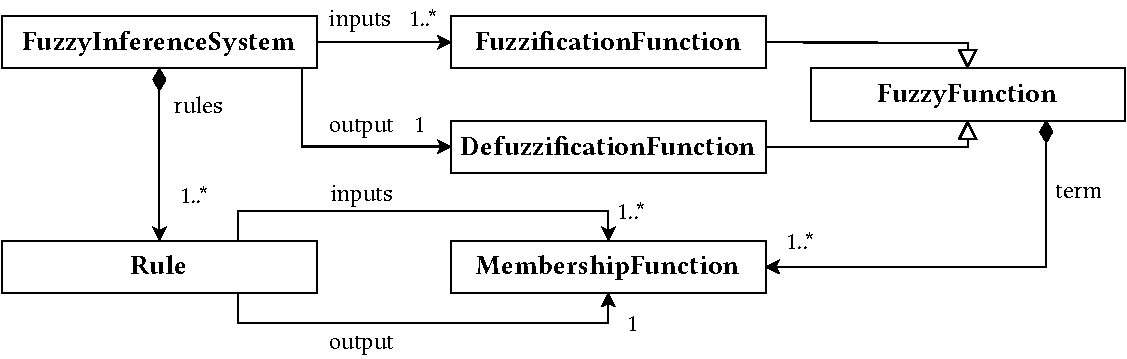
\includegraphics[width=\linewidth]{figures/chapter7/fis-metamodel.pdf}
    \caption{Excerpt from the class diagram of the \acf*{FIS} meta model.}
    \label{fig:confidentialityanalysis:fismetamodel}
\end{figure}

We present a \ac{FIS} metamodel as a way to enable software architects to create \acp{FIS}.
\autoref{fig:confidentialityanalysis:fismetamodel} shows an excerpt of the class diagram representation of the FIS metamodel. 
We represent the environmental factors as \emph{fuzzification functions}, which are made up of \emph{membership functions}. 
Each membership function defines a fuzzy set and represents a \emph{linguistic value} the environmental factor can take on. 
The corresponding membership functions define a degree of membership to the fuzzy set within an interval of $[0,1]$. 
Using the value of the environmental factor, e.g. a $30 \%$ signal-to-noise ratio, the fuzzifier calculates a degree of membership for each fuzzy set of the associated fuzzification function. 
In our running example, the signal-to-noise ratio can take on the linguistic values of \emph{low} and \emph{high}. 
The linguistic values of age are \emph{new} and \emph{old}.
As an example, the environmental factor values of a $30 \%$ signal-to-noise ratio would result in the membership degree of $0$ for \emph{high} and $0.5$ for \emph{low}. 
3 minutes of age would result in the membership degree of $0$ for \emph{new} and $1$ for \emph{old}.
Rules to combine the environmental factors are defined by combining a linguistic value of each environmental factor and defining a result. 
A rule that combines the most negative linguistic values of signal-to-noise ratio and age and consequently results in \emph{low} confidence is defined like this: \emph{IF signal-to-noise ratio is 'low' AND age is 'old' THEN confidence is 'low'}. 
Depending on how the \ac{FIS} is set up, the membership degrees of the linguistic values of a rule are combined. 
The result of the rule with the highest combined membership degrees is returned. 
Similar to how membership functions are used in the GuideArch approach \cite{esfahani_guidearch_2013}, a software architect can initially define the environmental factor value as a fuzzy set. 
In subsequent stages of development, when more information becomes available, these ranges can be narrowed down or fixed to a value. 
For our running example, this could be done by measuring the signal-to-noise ratio in the actual physical environment.

Using \acp{FIS} in the process has several benefits. 
\textcite{klir_fuzzy_1995} describe that through fuzzification an enhanced ability to model real-world problems is gained, lowering overall solution cost. 
The use of fuzziness also serves to better capture human common-sense reasoning and decision-making \cite{klir_fuzzy_1995}. 
When setting up a calculation rule in general, the system's properties and environment are abstracted and simplified. 
As a result, information about the inputs and their influence on the result is lost. 
A \ac{FIS} conserves more knowledge about the inputs and their influence on the calculated confidence value than a conventional mathematical function by mapping inputs to membership functions and working with natural language concepts. 
Additionally, a \ac{FIS} is capable of capturing the meanings of sentences in natural language \cite{klir_fuzzy_1995}, which enables, e.g., a software architect or security expert to easily map statements or requirements about the influence of environmental factors on confidence to calculation rules.

\begin{figure}
    \centering
    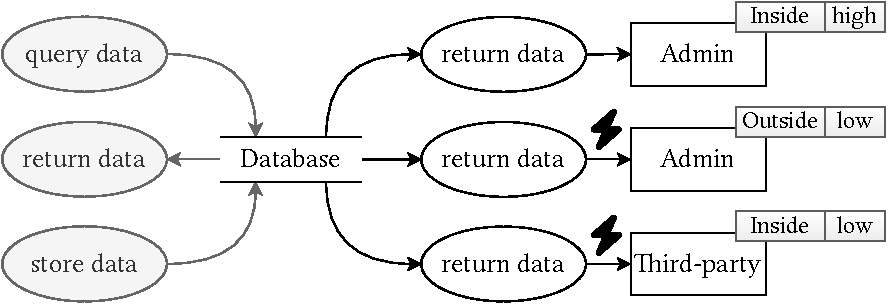
\includegraphics[width=0.95\linewidth]{figures/chapter7/dfd-environmental.pdf}
    \caption{\acf*{DFD} of the extended running example with additional actors and their node labels. Confidentiality violations are marked with lightning bolts.}
    \label{fig:confidentialityanalysis:dfdenvironment}
\end{figure}

We extend the data flow analysis presented in \autoref{sec:confidentialityanalysis:framework} to consider the so-calculated confidence values.
Here, we build on the representation of all confidentiality-related characteristics as data labels and node labels.
As confidence is directly related to such attributes, we extend these characteristics by adding confidence labels. 
\autoref{fig:confidentialityanalysis:dfdenvironment} shows a \ac{DFD} of the extension of our running example with simplified data flows to the actors.
The original data flows from the \emph{Customer} on the left are marked gray.
We add the node labels of the \emph{Admin} actors a third-party actors with their corresponding \emph{confidence} labels \emph{low} and \emph{heigh}.
As discussed previously, these confidence labels originate from the \ac{FIS} based on the input variables from the HSGPS or GPS sensors.
The confidentiality requirement is defined as a data flow constraint that only allows data to flow to actors within the building with \emph{high} confidence.
Thus, the upper data flow is permitted as the \emph{Admin} is inside the building with \emph{high} confidence.
The other data flows show confidentiality violations, as the \emph{Admin} is either outside the building, or a \emph{Third-Party} is considered to be inside the building with only \emph{low} confidence.
Without considering the confidence, the bottom confidentiality violation regarding the \emph{Third-Party} would be missed.

We include all calculated confidence labels in all node and data labels and also in the formulation of data flow constraints.
Although this represents a white-box extension of the data flow analysis, we do not alter the label propagation algorithm, only the textual representation of labels \cite{boltz_handling_2022}.
Thus, the calculation of the \ac{FIS} can be interpreted as a preprocessing step before the data flow analysis.
According to our classification, this represents a \emph{graph-aware} data flow analysis (\level{3}) under uncertainty.
The analysis result contains all information from the data flow analysis, e.g., violation location, violated data flows, and the mismatching labels that cause the violation, including information about the calculated confidence.
Due to the application of \acp{FIS}, information about both the environmental uncertainty sources and their impact is represented within the model and the analysis, as discussed previously.
Last, uncertainty can be analyzed independently on distinct data flows, which minimizes the analysis complexity.
For more information on the realization, please consult our publication \cite{boltz_handling_2022}, or the data set \cite{dataset}.

To conclude this section, we compare and discuss both approaches of uncertainty type-specific data flow analysis.
Both approaches employ already known techniques for representing and handling uncertainty \cite{sobhy_evaluation_2021,troya_uncertainty_2021}, i.e., design space exploration \cite{koziolek_peropteryx_2011,koziolek_automated_2011} or fuzzy inference \cite{klir_fuzzy_1995}.
Both approaches combine these techniques with data flow analysis, either in a black-box manner as in the first approach, or a white-box manner in the second approach.
This results in the first approach for structural uncertainty being \emph{scenario-aware} and the second approach for environmental uncertainty being \emph{graph-aware}.

Both approaches are type-specific and employ techniques that are suited for representing their targeted uncertainty type, i.e., design space exploration for structural uncertainty \cite{sobhy_evaluation_2021,troya_uncertainty_2021}, and fuzzy inference for environmental uncertainty \cite{cheng_fuzzy_2007,esfahani_guidearch_2013,hosmer_using_1992}.
Despite their differences in supported uncertainty types and realization, they show the commonality of considering uncertainty in form of scenarios.
The design decision model of PerOpteryx enables software architects to describe design alternatives, i.e., different scenarios of a software architecture.
The application of \acp{FIS} enables software architects to calculate distinct classes of a \emph{confidence} value, e.g., \emph{low} or \emph{high}, i.e., different scenarios describing the attributes in access control decisions.
The suitability of scenarios or variation \cite{walter_architecture-based_2023} to represent uncertainty has simultaneously been found by \textcite{troya_uncertainty_2021}.
However, besides being type-specific, both approaches also share the shortcoming of requiring expert knowledge.
Software architects or security experts have to instantiate the \ac{FIS} meta model with accurate values or have to specify design decision models.
In the following, we build on these findings to define uncertainty type-agnostic data flow analysis.

\finding{Data flow analysis can be extended by techniques like design space exploration or fuzzy inference to consider uncertainty within the analysis.
Here, decomposing uncertainty sources into their scenarios is expedient.}





\section{Uncertainty Type-Agnostic Data Flow Analysis}%
\label{sec:confidentialityanalysis:typeagnostic}

In this section, we present the second two approaches for uncertainty-aware data flow analysis.
The first approach is \emph{graph-aware} (\level{3}) and the second approach is \emph{impact-aware} (\level{4}), which represents the highest awareness level, see \autoref{sec:confidentialityanalysis:representing}.
Both approaches are type-agnostic, i.e., support all five uncertainty types introduced in \autoref{sec:classification:classification}.
We also present \abunai, which is tooling to support the modeling and analysis of the \emph{impact-aware} approach.
This addresses Problem \PR{3}{3} about type-agnostic data flow analysis.


\subsection{Tracing Uncertainty in Data Flow Analysis}%
\label{sec:confidentialityanalysis:tracing}

Incorporating information about independent data flows---called \acp{TFG} in our terminology introduced in \autoref{sec:confidentialityanalysis:framework}---enables the definition of \emph{graph-aware} analysis (\level{3}).
We present an analysis that traces confidentiality violations back to the originating uncertainty sources using this information.
This enables relating violations to concrete scenarios and simplifies the interpretation and mitigation by software architects.

In this approach, we use variation models \cite{walter_architecture-based_2023,mehl_palladio_2022} to express uncertainty sources and their scenarios.
Variation models are similar to the already discussed design decision models presented in \autoref{sec:confidentialityanalysis:typespecifc}.
Software architects specify target elements and alternative elements of the software architecture.
This can be applied, for instance, to deployment locations, or to actions in \acfp{SEFF}.
As discussed previously, \emph{design uncertainty} is \enquote{normally represented in software models by variability models} \cite{troya_uncertainty_2021}.
Model variation can be used to describe possible outcomes of \emph{Scenario Uncertainty}.
Each uncertainty is represented by a variation point and a selection of alternative architectural elements.
This description results in a variation model \cite{mehl_palladio_2022} of the software architecture.
\autoref{table:confidentialityanalysis:scenarios} shows all scenarios of all uncertainties of the running example.

Based on the variation model, architectural variants can be generated by permutation \cite{mehl_palladio_2022}.
If the information about data flows were ignored, this would cause the same complexity as a \emph{scenario-aware} analysis (\level{2}).
As discussed in \autoref{sec:confidentialityanalysis:representing}, our running example requires $48$ variations.
However, not all uncertainties affect all \acp{TFG}.
Thus, the relevant variations can be filtered in \emph{graph-aware} analysis (\level{3}).
The resulting variants are then analyzed by the data flow analysis presented in \autoref{sec:confidentialityanalysis:framework}.
By relating the resulting confidentiality violations to the analyzed variation and its uncertainty, software architects can focus on critical variants, i.e., variants that violate confidentiality.
The hereby defined analysis traces violations back to their originating uncertainties \cite{bitschi_uncertainty-aware_2022}.

\begin{table}
    \centering
    \begin{tabular}{lll}
        \toprule
        \# & \ac{TFG} name & Relevant uncertainty sources\\
        \midrule
        1 & Request support contact & -  \\
        2 & View available items & \U{3}, \U{4} \\
        3 & Purchase items & \U{1}, \U{2}, \U{3}, \U{4} \\
        \bottomrule
    \end{tabular}
    \caption{Relation of \acfp*{TFG} and uncertainty sources in the running example.}%
    \label{table:confidentialityanalysis:scenariostfgs}
\end{table}

\autoref{table:confidentialityanalysis:scenariostfgs} shows the three \acp{TFG} in the running example and the uncertainty sources that can be found in these \acp{TFG}.
This table can be derived based on \autoref{fig:runningexample:dfd} showing the \ac{DFD} of the running example and \autoref{table:confidentialityanalysis:scenarios} showing the scenarios of all uncertainty sources.
The first \ac{TFG} representing the support contact request is not affected by uncertainty.
The second \ac{TFG} is only affected by the deployment (\U{3}) and the provider trustworthiness (\U{4}).
The third \ac{TFG} is additionally affected by the user input (\U{1}) and the data processing (\U{2}), i.e., by all uncertainties in the running example.

As the three \acp{TFG} are independent, their variations can be analyzed independently.
This results in the lowered complexity of the \emph{graph-aware} analysis (\level{3}) compared to the \emph{scenario-aware} analysis (\level{2}).
Instead of having to apply all possible variations to each \ac{TFG}, we can first filter the relevant uncertainty sources and then only analyze all variations of these uncertainty sources.
Note that this does not affect the identified confidentiality violations as the data flows represented by the \acp{TFG} are independent \cite{seifermann_architectural_2022}.
While the complexity is reduced, the accuracy remains the same.
The more independent data flows there are, the greater this effect becomes, as we assume in real software systems \cite{hahner_architecture-based_2023}.

\begin{algorithm}
    \caption{Algorithm for graph-aware data flow analysis under uncertainty}
    \label{alg:confidentialityanalysis:graphaware}
    \begin{algorithmic}[1]
        \Procedure{\function{analyzeGraphAware}}{$\var{model}, \var{constraint}, \var{uncertainties}$}
            \algindentskip
            \State $\var{violations} \gets \emptyset$
            \State $\var{filtered} \gets \emptyset$
            \State $\var{variations} \gets \function{generateAllVariations}(\var{model}, \var{uncertainties})$
            \State $\var{tfgs} \gets \function{retrieveAllTFGs}(\var{model})$
            \algblockskip

            \For{$\var{tfg} \in \var{tfgs}$} \Comment{Analyze each TFG separately} \label{alg:confidentialityanalysis:graphaware:6}
                \For{$\var{variation} \in \var{variations}$} \Comment{Filter relevant variations}
                    \State $\var{filtered} \gets \var{filtered} \cup \function{filterVariation}(\var{model}, \var{tfg}, \var{variation}, \var{uncertainties})$\label{alg:confidentialityanalysis:graphaware:8}
                \EndFor
                \algblockskip

                \For{$\var{variation} \in \var{filtered}$} \Comment{Only analyze filtered variations}
                    \State $\var{modifiedtfg} \gets \function{applyVariation}(\var{tfg}, \var{variation})$ \label{alg:confidentialityanalysis:graphaware:11}
                    \State $\var{violations} \gets \var{violations} \cup \function{analyze}(\var{modifiedtfg}, \var{constraint})$ 
                \EndFor
            \EndFor
            \algblockskip

            \State \Return{$\var{violations}$}
            \algindentskip
        \EndProcedure   
    \end{algorithmic}
\end{algorithm}

\autoref{alg:confidentialityanalysis:graphaware} shows the algorithm for \emph{graph-aware} data flow analysis (\level{3}).
The approach is similar to \emph{scenario-aware} data flow analysis shown in \autoref{alg:confidentialityanalysis:scenarioaware}, but comprises the aforementioned filtering.
We iterate over all \acp{TFG} of a model in \autoref{alg:confidentialityanalysis:graphaware:6} and analyze each \ac{TFG} separately.
This is possible because \emph{graph-aware} analysis has the information of all data flows.
For each \ac{TFG}, we filter the variations for relevant ones in \autoref{alg:confidentialityanalysis:graphaware:8}.
Afterward, we run the analysis only on these variations.
This is achieved by applying the variation first in \autoref{alg:confidentialityanalysis:graphaware:11} and then forwarding the \ac{TFG} to the data flow analysis.

\begin{algorithm}
    \caption{Algorithm for filtering variations in graph-aware analysis}
    \label{alg:confidentialityanalysis:filtervariation}
    \begin{algorithmic}[1]
        \Procedure{\function{filterVariation}}{$\var{model}, \var{tfg}, \var{variation}, \var{uncertainties}$}
            \algindentskip

            \State $\var{applied} \gets \function{getAppliedUncertainties}(\var{variation, \var{uncertainties})}$ \label{alg:confidentialityanalysis:filtervariation:4}
            \State $\var{vertices} \gets \function{getVertices}(\var{tfg})$ \Comment{Iterate over all vertices}
            \For{$\var{vertex} \in \var{vertices}$} \label{alg:confidentialityanalysis:filtervariation:6}
                \For{$\var{uncertainty} \in \var{applied}$}
                    \If{$\function{affects}(\var{uncertainty}, \var{vertex}, \var{model}, \var{variation})$} \label{alg:confidentialityanalysis:filtervariation:8}
                        \State $\var{applied} \gets \var{applied} \setminus \setted{\var{uncertainty}}$ \label{alg:confidentialityanalysis:filtervariation:9}
                    \EndIf
                \EndFor
                \algblockskip

                \If{$\var{applied} = \emptyset$} \Comment{All uncertainties are relevant}
                    \State \Return{$\setted{\var{variation}}$} \label{alg:confidentialityanalysis:filtervariation:13}
                \EndIf
            \EndFor
            \algblockskip

            \State \Return{$\emptyset$} \label{alg:confidentialityanalysis:filtervariation:17} \Comment{At least one uncertainty is not relevant}
            \algindentskip
        \EndProcedure   
    \end{algorithmic}
\end{algorithm}

\autoref{alg:confidentialityanalysis:filtervariation} shows this filter function.
A variation is relevant for a given \ac{TFG} if all uncertainty sources that cause a change in the architectural model affect at least on vertex of the \ac{TFG}.
We start by retrieving all uncertainties that have been applied in the given variation in \autoref{alg:confidentialityanalysis:filtervariation:4}.
This is the case, if the permutation that causes the variation \cite{mehl_palladio_2022} changes an architectural element due to said uncertainty.
For instance, if one variation only changes architectural elements representing the data processing and the deployment location in our running example, this function would yield the uncertainties \U{2} and \U{3}.
Note that this function is called with \emph{all} possible variations calculated in \autoref{alg:confidentialityanalysis:graphaware}.

Afterward, we iterate over all vertices of the \ac{TFG} in \autoref{alg:confidentialityanalysis:filtervariation:6}.
For each applied uncertainty, we check whether this uncertainty affects the current vertex in \autoref{alg:confidentialityanalysis:filtervariation:8}.
An uncertainty affects a vertex \emph{iff} it causes a variation in an architectural element that is represented by the vertex.
The underlying mapping of the data flow analysis framework presented in \autoref{sec:confidentialityanalysis:framework} is similar to the mapping between architectural models and \acp{DFD} discussed in \autoref{sec:impactanalysis:impactanalysis}.
In our running example, uncertainty in the data processing (\U{2}) affects all vertices in all \acp{TFG} representing this data processing.
If we find such an uncertainty \emph{impact}, we remove the uncertainty from the list of applied uncertainties in \autoref{alg:confidentialityanalysis:filtervariation:9}.

The procedure ends if, at any point in the iteration over all vertices of a \ac{TFG}, the list of applied uncertainties gets empty.
This is the case if all uncertainties considered in the given variation are relevant to the \ac{TFG}.
Thus, the variation is relevant for the \emph{graph-aware} analysis and is returned in \autoref{alg:confidentialityanalysis:filtervariation:13}.
If not all uncertainties that have been varied are relevant, an empty set is returned instead in \autoref{alg:confidentialityanalysis:filtervariation:17}.

We explain the interplay of \autoref{alg:confidentialityanalysis:graphaware} and \autoref{alg:confidentialityanalysis:filtervariation} based on the the three \acp{TFG} of our running example, shown in \autoref{table:confidentialityanalysis:scenariostfgs}.
Here, the analyzing the first \ac{TFG} representing the support contact request and the last \ac{TFG} representing the item purchase are the edge cases of the filter algorithm.
The first \ac{TFG} has no relevant uncertainty source.
Thus, \autoref{alg:confidentialityanalysis:filtervariation} always returns an empty list except for the single variation, where no uncertainty is applied.
In this case, \autoref{alg:confidentialityanalysis:filtervariation:8} trivially evaluates to \emph{true} as the list already was empty.
The third \ac{TFG} is affected by all four uncertainty sources \U{1} -- \U{4}.
Thus, every permutation of the uncertainties creates a variation that is relevant for the \ac{TFG} and the filter has no effect.
Regarding the second \ac{TFG}, only four variations are relevant, i.e., the variations that represent the scenarios of Uncertainty \U{3} and Uncertainty \U{4}, \autoref{table:confidentialityanalysis:scenariostfgs}.
Only these variations are returned by the filter algorithm and analyzed using the data flow analysis.
This also again shows the reduced complexity of the \emph{graph-aware} analysis (\level{3}), as for most \acp{TFG} in the running example, not all variations are relevant.

The information about uncertainty sources, filtered variations, \acp{TFG}, and confidentiality violations enables the tracing approach.
For each confidentiality violation, we can store the related \ac{TFG} and which variation has been applied in the analysis process.
The reference to the variation provides the knowledge about considered uncertainty sources and their properties.
This represents the information categories \textbf{1.} -- \textbf{8.} from \autoref{table:confidentialityanalysis:informationcategories}.
Combined, this provides software architects with comprehensive knowledge to better understand the origin of the confidentiality violations and to apply appropriate measures.

\begin{figure}
    \centering
    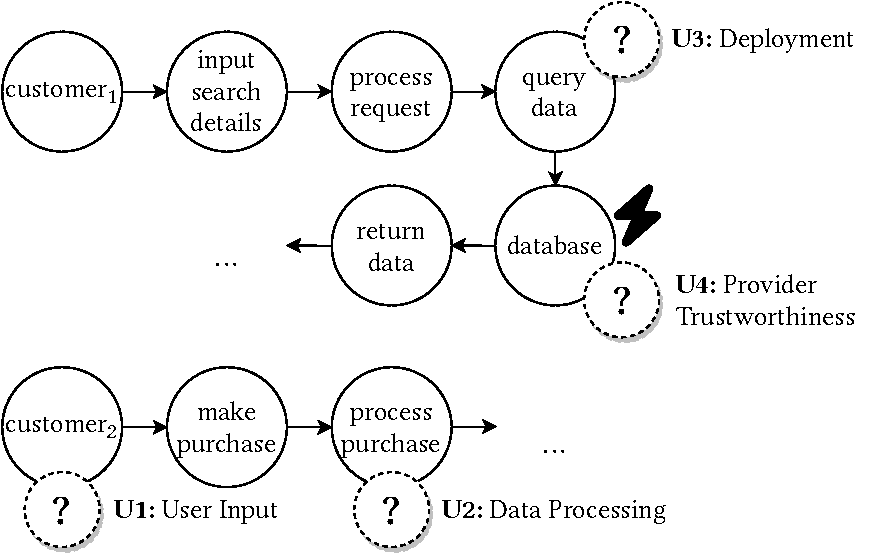
\includegraphics[width=0.95\linewidth]{figures/chapter7/uncertaintytracing.pdf}
    \caption{Excerpts of two \acfp*{TFG} from the running example with annotated uncertainty impacts and a confidentiality violation, marked with a lightning bolt.}
    \label{fig:confidentialityanalysis:uncertaintytracing}
\end{figure}

We illustrate this with one variation of the uncertainty sources of the running example.
\autoref{fig:confidentialityanalysis:uncertaintytracing} shows excerpts of the \acp{TFG} that represent the querying of items and the making of purchases.
The annotated uncertainty represents the impact of the uncertainty due to changes in the architectural model.
For instance, in this variation, the deployment location is the \emph{Cloud Service} and the provider is classified as \emph{Suspicious}, see \autoref{table:confidentialityanalysis:scenarios}.
This uncertainty would cause a confidentiality violation when the data is stored in the database, as marked with the lightning bolt.
As discussed with \autoref{table:confidentialityanalysis:scenariostfgs}, this represents one of the $48$ possible variations.
This confidentiality violation can thus be traced back to the uncertainties \U{3} and \U{4}.
The tracing follows the data flow in inverse direction, and could thus be interpreted as a reverse uncertainty impact analysis.
The graphical representation of the \acp{TFG} in \autoref{fig:confidentialityanalysis:uncertaintytracing} also shows the independence to the other uncertainty sources, e.g., \U{1}, and \U{2}.
They affect other vertices of another \ac{TFG} and can thus be safely ignored when interpreting the confidentiality violation in the upper \ac{TFG}.
This benefits the understanding of software architects and simplifies both further analyses and the mitigation.

\emph{Graph-aware} data flow analysis (\level{3}) minimizes the analysis complexity while enhancing the expressiveness of the analysis results.
As the presented approach for tracing uncertainty builds on variation modeling \cite{mehl_palladio_2022,walter_architecture-based_2023}, any architectural element can be varied.
This enables an uncertainty type-agnostic approach.
However, this approach has two major shortcomings.
First, variation modeling still requires some expert knowledge from the software architects.
Although they do not have to manually model the variations or alter the \acp{DFD} by hand, they have to specify the correct variation types and variation points.
This requires them to understand which variation points match the uncertainty sources they want to analyze.
Failing to accurately represent the uncertainty in the variation model can impair or even void the analysis results \cite{hahner_arcn_2024}.
This discussion is similar to the extension of the uncertainty impact analysis shown in \autoref{sec:impactanalysis:awareness}.

Second, the approach ignores uncertainty interactions.
For instance, if the \emph{Database Service} is deployed on-premise, Uncertainty \U{4} about the provider's trustworthiness has no effect.
Because the uncertainty filter presented in \autoref{alg:confidentialityanalysis:filtervariation} does not consider this, more varied \acp{TFG} are analyzed than required.
In this example, the variation of a \emph{suspicious} cloud provider and a deployment \emph{on premise} can be safely ignored as there would be no data flow to the cloud provider in the first place.
This marks the difference between a \emph{graph-aware} analysis (\level{3}) and an \emph{impact-aware} analysis (\level{4}).
The difference becomes visible when comparing \autoref{fig:classification:dag} with \autoref{fig:confidentialityanalysis:uncertaintytracing}.
The former shows uncertainty as part of the \ac{DFD} while the latter only considers changes in architectural elements that are related to \ac{DFD} nodes.
Generating and filtering variations cannot represent transitive effects of uncertainty impacts within a \ac{DAG}.
To address this, we consider uncertainty as a first-class concern in the data flow analysis, creating an \emph{impact-aware} analysis (\level{4}).

\finding{Considering \acfp{TFG} in the confidentiality analysis of uncertainty scenario combinations surpasses the analysis capabilities of analyses that only consider all possible variations.
Still, the resulting analysis is limited by the expressiveness of variation modeling.
To overcome this limitation regarding the transitive impact, uncertainty has to be presented as first-class concern within \acfp{DFD} and the data flow analysis.}


\subsection{Impact-Aware Data Flow Analysis Under Uncertainty}%
\label{sec:confidentialityanalysis:abunai}

More than a decade ago, \textcite{garlan_software_2010} proposed to consider uncertainty as a first-class concern in software engineering.
We follow this proposal to define the last approach of this chapter, an uncertainty type-agnostic and \emph{impact-aware} data flow analysis (\level{4}).
First, we present a meta model for representing uncertainty sources as part of the architectural model.
This addresses the shortcoming regarding expert knowledge of variation modeling \cite{mehl_palladio_2022,walter_architecture-based_2023,hahner_model-based_2023}.
Afterward, we introduce the notion of a \acf{NDFD} \cite{hahner_classification_2023} that incorporates uncertainty as a first-class entity within the \ac{DFD}.
We discuss how to analyze such \acp{NDFD} and handle simple uncertainty interactions in \acp{DAG} while identifying confidentiality violations.
Last, we present our tooling \abunai that comprises uncertainty modeling and automated analysis support.

In presenting the previous approaches for analyzing structural uncertainty and environmental uncertainty, and tracing uncertainty, we discussed different approaches to express uncertainty as part of the architectural model.
This includes design decision models \cite{koziolek_peropteryx_2011,koziolek_automated_2011,walter_architectural_2022}, \acp{FIS} \cite{klir_fuzzy_1995,boltz_handling_2022}, and variation modeling \cite{mehl_palladio_2022,hahner_model-based_2023}.
They share the common shortcoming of requiring expert knowledge to bridge the gap between identifying uncertainty sources and expressing them as part of the software architecture.
We close this gap by providing a meta model that connects the five uncertainty types presented in \autoref{ch:classification} to the architectural model.
This approach is similar to the modeling of uncertainty for impact analysis presented in \autoref{sec:impactanalysis:representing}, where we already addressed a similar issue.

\begin{figure}
    \centering
    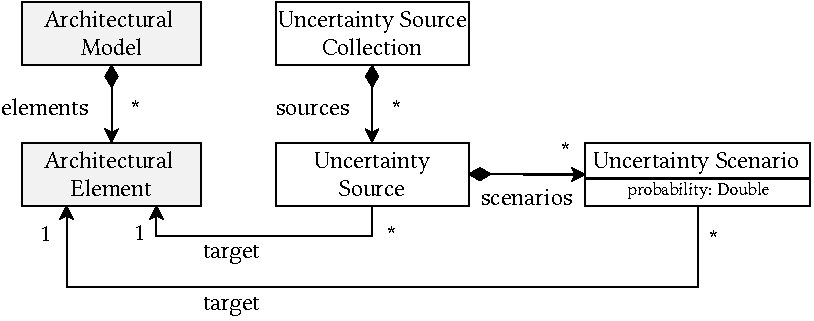
\includegraphics[width=0.95\linewidth]{figures/chapter7/abunai-metamodel.pdf}
    \caption{Overview of the meta model for expressing uncertainty sources and scenarios in architectural models. Existing elements of the software architecture are highlighted gray.}
    \label{fig:confidentialityanalysis:uncertaintymetamodel}
\end{figure}

\autoref{fig:confidentialityanalysis:uncertaintymetamodel} shows the meta model for modeling uncertainty sources and scenarios as part of the software architecture.
We use the same terminology as the uncertainty classification presented in \autoref{ch:classification}, i.e., uncertainty sources and scenarios, instead of design decisions, or variations.
To introduce this meta model, we only refer to the concept of an \emph{Architectural Model}, which comprises any number of \emph{Architectural Elements}.
Software architects define an \emph{Uncertainty Source Collection} alongside the architectural model.
This collection consists of \emph{Uncertainty Sources} that consist of \emph{Uncertainty Scenarios}.
Each source references one \emph{Architectural Element}, which represents its default scenario.
Until this point, the software architecture is annotated with uncertainty sources like in the uncertainty impact analysis, see \autoref{ch:impactanalysis}.
We extend this annotation by modeling any number of \emph{Uncertainty Scenario} that also refer to one \emph{Architectural Element}.
These scenarios represent alternative scenarios of the \emph{Uncertainty Source} any can additionally have a probability.

\begin{figure}
    \centering
    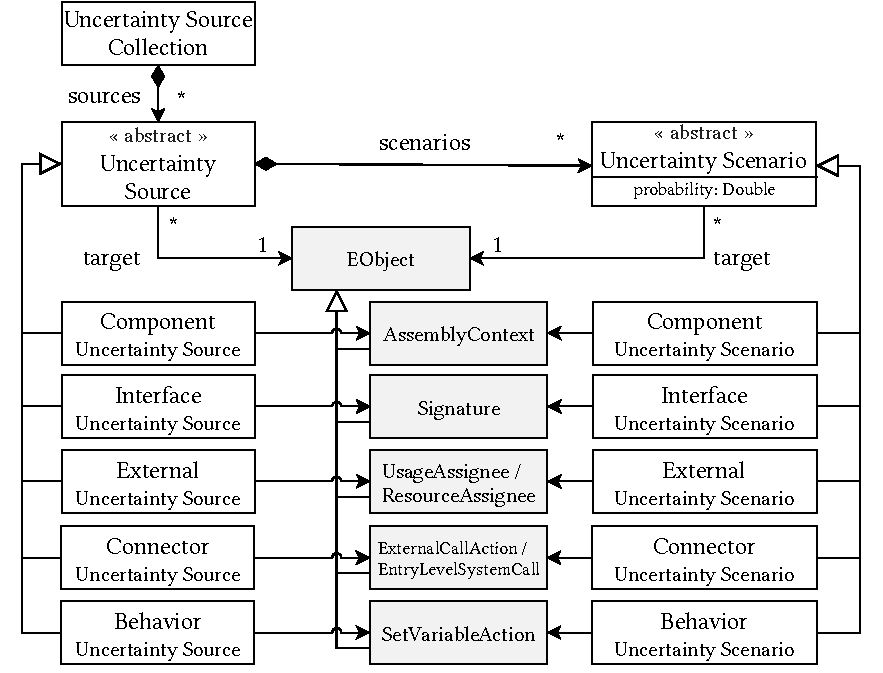
\includegraphics[width=\linewidth]{figures/chapter7/abunai-metamodel-pcm.pdf}
    \caption{Meta model of uncertainty sources and scenarios in the \acf*{PCM}.}
    \label{fig:confidentialityanalysis:uncertaintymetamodelpcm}
\end{figure}

Depending on the type of modeled uncertainty, see \autoref{table:classification:classification:type}, software architects can refine the model.
\emph{Recognized Ignorance} is modeled as an \emph{Uncertainty Source} that references an \emph{Architectural Element}.
\emph{Scenario Uncertainty} is modeled as a \emph{Uncertainty Source} with any number of \emph{Uncertainty Scenarios} that also reference \emph{Architectural Elements}.
\emph{Statistical Uncertainty} is modeled by enriching the \emph{Uncertainty Scenarios} with probabilities between 0 and 1.
We require that all probabilities add up to 1.
The probability of the default scenario expressed by the \emph{Uncertainty Source} is 1 minus the sum of the probabilities of all of its scenarios.
However, providing probabilities is optional, the field can be left empty to describe \emph{Scenario Uncertainty}.
Depending on the available information, all options of the category \emph{Uncertainty Type} presented in \autoref{sec:classification:classification} can be modeled and mixed.
In our running example, Uncertainty \U{4} is modeled by creating an \emph{Uncertainty Source} that refers to the \emph{Cloud Service's} trustworthiness with the alternative \emph{Uncertainty Scenario} of being suspicious, see \autoref{table:confidentialityanalysis:scenarios}.
A high level of trust in the provider can be expressed, for example, by a probability of 0.1 for the alternative scenario of a suspicious provider.

We extend this meta model and apply it to the \ac{PCM}, thereby replacing the \emph{Architectural Elements} of \autoref{fig:confidentialityanalysis:uncertaintymetamodel} with concrete \ac{PCM} element types.
\autoref{fig:confidentialityanalysis:uncertaintymetamodelpcm} shows the resulting meta model.
We simplify some of the elements for the sake of clarity, e.g. by combining \emph{UsageAssignees} and \emph{ResourceAssignees}, which are modeled separately.
Similarly to the overview, a \emph{Uncertainty Source Collection} contains any number of \emph{Uncertainty Sources} that contain any number of \emph{Uncertainty Scenarios}.
Both the \emph{Uncertainty Source} and the \emph{Uncertainty Scenario} target exactly one architectural element.
Because the \ac{PCM} is based on the \acf{EMF}, the common super type is \emph{EObject}.

The five uncertainty types of the category \emph{Architectural Element Type}, see \autoref{table:classification:classification:architecturalelementtype}, have their corresponding uncertainty sources and uncertainty scenarios.
All sources inherit from the abstract \emph{Uncertainty Source} and all scenarios from the abstract \emph{Uncertainty Scenario}, respectively.
For the sake of clarity, we leave out details like the inherited \emph{probability} field and the \emph{scenarios} relation between all sub types.
All sources and scenarios target an \ac{PCM} element type, e.g., \emph{Component Uncertainty Sources} and \emph{Component Uncertainty Scenarios} target \ac{PCM} \emph{AssemblyContexts}.
This ensures valid model instances, as both sources and scenarios are required to reference the same \ac{PCM} element type, e.g., different \emph{AssemblyContexts}, or \emph{Signatures}.
Some types of \emph{Uncertainty Sources} and \emph{Uncertainty Scenarios} can refer to more than one \ac{PCM} element, e.g., \emph{Connector} uncertainty, and \emph{External} uncertainty.
In our implementation of this meta model \cite{dataset}, we realize this using sub types of \emph{Connector} uncertainty and \emph{External} uncertainty, respectively, to ensure type safety.
Note that the referenced \ac{PCM} elements are slightly different compared to the annotated elements of uncertainty impact analysis, as discussed in \autoref{sec:impactanalysis:representing}.

\begin{table}
    \begin{tabularx}{\linewidth}{lllX}
        \toprule
        \# & Uncertainty type & Source target \ac{PCM} element & Alternative scenario targets \\
        \midrule
        \U{1} & Connector & \emph{BuyEntryLevelSystemCall} & 
            \mtl{\emph{ErroneousEntryLevelSystemCall}\\\emph{MaliciousEntryLevelSystemCall}} \\
        \U{2} & Behavior & \emph{UserDataProcessing} & 
            \mtl{\emph{BrokenEncryptionProcessing}\\\emph{BrokenValidationProcessing}\\\emph{EverythingBrokenProcessing}} \\
        \U{3} & Component & \emph{DatabaseServiceOnPremise} & \emph{DatabaseServiceInCloud} \\
        \U{4} & External & \emph{ProviderTrusted} & \emph{ProviderSuspicious} \\
        \bottomrule
    \end{tabularx}
    \caption{Modeling the uncertainty sources and their scenarios in the running example.}%
    \label{table:confidentialityanalysis:uncertaintymodelrunningexample}
\end{table}

We apply this meta model to our running example to illustrate it with all uncertainty sources \U{1} -- \U{4}.
\autoref{table:confidentialityanalysis:uncertaintymodelrunningexample} shows the targeted elements of all uncertainty sources and also the targeted elements of alternative scenarios.
Thereby it realizes the scenarios \autoref{table:confidentialityanalysis:scenarios} and connects this collection to a concrete architectural model described based on the \ac{PCM}.
The restriction to concrete architectural elements simplifies the modeling of uncertainty sources and their scenarios and also minimizes the risk of an erroneous specification.
Compared to, e.g., variation modeling \cite{mehl_palladio_2022,walter_architecture-based_2023}, this bridges the gap between the classification of software-architectural uncertainty and the software architecture.

\finding{Modeling uncertainty sources and uncertainty scenarios that reference elements of the architectural model connects the classification of software-architectural uncertainty to architectural models.
This provides the foundation for analyzing uncertainty as first-class entity in software architecture.}

To consider uncertainty not only as first-class entity within the software architecture but also in architecture-based data flow analysis, we need means to represent the impact in \acp{DFD}.
To this end, we discussed the mapping and the representation of uncertainty to \acp{DFD} and \acp{DAG} in \autoref{sec:classification:dfd}.
We also introduced the notion of \emph{primary} uncertainty that affects vertices and \emph{secondary} uncertainty that affects edges.
By connecting this notion to the previously introduced meta model for modeling uncertainty sources and scenarios, we are able to define an \emph{impact-aware} data flow analysis (\level{4}).
Uncertainty is sometimes defined as \enquote{any departure from the unachievable ideal of complete determinism} \cite{walker_defining_2003}, see \autoref{sec:foundations:uncertainty}.
We build on this idea by describing the lack of determinism and define the notion of \acfp{NDFD}.
Put simply, we extend \acfp{DFD} to incorporate uncertainty as first-class entity that is represented by nondeterminism.
Here, we also benefit from the comprehensive foundations regarding the representation of the impact of uncertainty in \ac{DFD}, provided in \autoref{sec:impactanalysis:representing}.

\begin{figure}
    \centering
    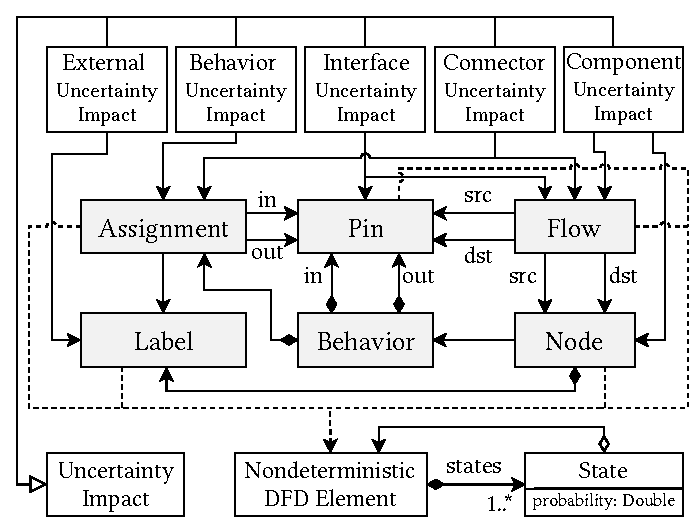
\includegraphics[width=0.8\linewidth]{figures/chapter7/ndfd.pdf}
    \caption{Meta model of \acfp*{NDFD}.}
    \label{fig:confidentialityanalysis:ndfd}
\end{figure}

\autoref{fig:confidentialityanalysis:ndfd} shows the meta model of \acp{NDFD}, thereby extending the meta model of \acp{DFD} with uncertainty impacts shown in \autoref{fig:impactanalysis:representing:metamodel}.
Every \ac{DFD} element originating from the unified modeling primitives \cite{seifermann_unified_2021} and highlighted in gray represents a \emph{Nondeterministic Data Flow Diagram Element}.
Such an element has one or more \emph{States} that reference the element, or other elements.
Trivially, an element with only one \emph{State} that references the element itself represents determinism.
Thus, every \ac{DFD} is also a valid \ac{NDFD}, which lacks nondeterminism, i.e., uncertainty.
Uncertainty is represented by multiple \emph{States} that can additionally have a \emph{probability}.
Regarding the probability, the same rules apply as for the meta model for uncertainty and scenarios in the architectural model.

This meta model enables the concise representation of uncertainty in \acp{DFD}.
For instance, Uncertainty \U{4} about the provider trustworthiness represents \emph{External} uncertainty.
It can be expressed by an nondeterministic \emph{Label} with two states: \emph{Trustworthy} and \emph{Suspicious}.
The same applies to the other uncertainty sources, e.g., Uncertainty \U{2} about the processing can be represented by multiple alternative \emph{Assignments}.

We reuse the mapping of uncertainty sources to impact locations within the \ac{DFD} from \autoref{sec:classification:dfd}, and the mapping of \ac{PCM} models to \acp{DFD} presented in \autoref{sec:confidentialityanalysis:framework}.
Additionally, every \emph{Uncertainty Scenario} from the meta model presented in \autoref{fig:confidentialityanalysis:uncertaintymetamodelpcm} is mapped to a \emph{State} of the \ac{NDFD} meta model.
The state representing the default scenario of the \emph{Uncertainty Source} references the \ac{DFD} element itself.
All alternative scenarios reference the \ac{DFD} elements that represent the targeted architectural elements of these scenarios.
The probability of a \emph{State} corresponds to the probability of the \emph{Uncertainty Scenario}.

We can apply this mapping to the modeled uncertainty sources and uncertainty scenarios of the running example, shown in \autoref{table:confidentialityanalysis:uncertaintymodelrunningexample}.
The \emph{EntryLevelSystemCall} that is referenced by Uncertainty \U{1} is mapped to a nondeterministic \ac{DFD} element and referenced by the default state of this element.
The \ac{DFD} element has additional states to also represent erroneous and malicious user input.
Because Uncertainty \U{1} represents \emph{Connector} uncertainty, the nondeterministic \ac{DFD} elements are flows and assignments that set the labels for valid, erroneous, or malicious input.
However, due to the uncertainty, we cannot know which assignment is applied, i.e., nondeterminism.

\finding{\acfp{NDFD} consist of all \acfp{DFD} elements, which have one or multiple states.
These states represent uncertainty as a first-class concern in modeling and data flow analysis.}

The concept of states in \acp{NDFD} can be transferred to \acp{DAG}.
This enables the application of the data flow analysis that operates on \acp{TFG}, which are \acp{DAG}.
Here, we use the notion of \emph{primary} and \emph{secondary} uncertainty.
As discussed in \autoref{sec:classification:dfd}, the five uncertainty types can be represented by either \emph{primary} or \emph{secondary} uncertainty.
\emph{Component} uncertainty, \emph{Connector} uncertainty, and \emph{Interface} uncertainty affect the data flow, i.e., the edges of a \ac{DAG}.
\emph{External} uncertainty and \emph{Behavior} uncertainty affect nodes, i.e., the vertices of a \ac{DAG}.
We use this mapping of the elements of a \ac{DFD}---that are also elements of a \ac{NDFD}---to simplify the data flow analysis.
In mapping \ac{PCM} elements to \acp{TFG}, we map the uncertainty sources and scenarios to \emph{primary} and \emph{secondary} uncertainty.
The resulting \ac{DAG} with these uncertainties represents a \ac{NDFD} and comprises uncertainty as a first-class entity.
To repeat from \autoref{sec:classification:dfd}, a \ac{DAG} $G = (V, E)$ consists of vertices $V$ and edges $E$.
All \emph{primary} uncertainty impacts form a subset of all vertices $V_{u} \subseteq V$.
All \emph{secondary} uncertainty impacts form a set $E_{u} = \setted{E_{u_{1}}, \dots, E_{u_{n}}}$, where each set comprises alternative edges.

\begin{figure}
    \centering
    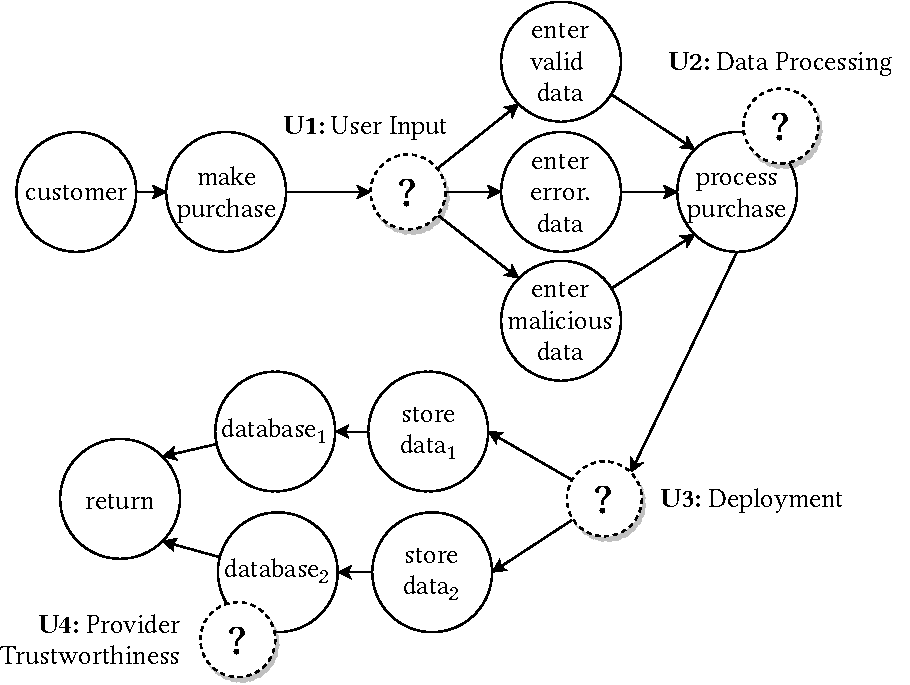
\includegraphics[width=0.9\linewidth]{figures/chapter7/lastdag.pdf}
    \caption{\acf*{DAG} of the \acf*{TFG} representing the item purchase in the running example, with primary and secondary uncertainty, denoted by question marks.}
    \label{fig:confidentialityanalysis:dag}
\end{figure}

The first \ac{TFG} of the support contact request contains no uncertainty and is thus not relevant, see \autoref{table:confidentialityanalysis:scenariostfgs}.
The \ac{DAG} of the second \ac{TFG} is shown while discussing \emph{primary} and \emph{secondary} uncertainty in \autoref{fig:classification:dag}.
To make the list of \acp{DAG} of the running example complete, \autoref{fig:confidentialityanalysis:dag} shows the \ac{DAG} of the third \ac{TFG} of the running example, which represents the purchase of items.
This \ac{DAG} contains all four uncertainties \U{1} -- \U{4}.

The \emph{secondary} uncertainties are shown as alternative edges.
As discussed above, the \emph{Connector} uncertainty of the user input (\U{1}) and the \emph{Component} uncertainty of the deployment (\U{3}) represent \emph{secondary} uncertainty.
The \emph{primary} uncertainties are annotated to vertices.
The \emph{Behavior} uncertainty of the data processing (\U{2}) and the \emph{External} uncertainty of the provider trustworthiness (\U{4}) represent \emph{primary} uncertainty.
The scenarios of the \emph{secondary} uncertainty are visible in the graphical representation of the \ac{DAG}, e.g., the alternative types of user input in Uncertainty \U{1}.
The scenarios of \emph{primary} uncertainty are hidden in this view, because they affect \ac{DFD} elements that are represented by the vertices, e.g., the \emph{Label} of the \emph{database\textsubscript{2}} being \emph{Trustworthy}, or \emph{Suspicious}.
Here, we refer to \autoref{sec:confidentialityanalysis:framework} for our introduction on \acp{TFG} and their relation to \acp{DAG}.

The \ac{TFG} shown in \autoref{fig:classification:dag} is also suitable to illustrate the mapping from an architectural model with uncertainty sources and scenarios to \acp{NDFD} and \acp{DAG}.
\autoref{table:confidentialityanalysis:uncertaintymodelrunningexample} shows three different scenarios regarding Uncertainty \U{1} of the user input.
As this is \emph{Connector} uncertainty and modeled with three alternative \emph{EntryLevelSystemCalls}, the resulting \ac{DAG} also comprises the corresponding vertices, e.g., \emph{enter valid data} and \emph{enter malicious data}, with a \emph{secondary} uncertainty.
In the \ac{NDFD}, this is represented by a nondeterministic element with three states, which translates to this part of the \ac{DAG}.
The same applies to Uncertainty \U{3} with the two deployment options.
The \emph{primary} uncertainties \U{2} and \U{4} have been discussed in the previous paragraph.
Here, the scenarios are not visible in the \ac{DAG}, because it only represents the \emph{Nodes} of an \ac{NDFD} as vertices, and \emph{primary} uncertainty affects these vertices.
Nevertheless, the label propagation presented in \autoref{sec:confidentialityanalysis:framework}, is presented with alternative \ac{DFD} elements, e.g., alternative \emph{Assignments} representing the data processing alternatives in Uncertainty \U{2}.
In sum, the notion of \acp{TFG} remains suitable to model and analyze \ac{DAG}, also under uncertainty.

We build on this representation of \acp{NDFD} as \emph{primary} and \emph{secondary} uncertainty in \acp{DAG} to define \emph{impact-aware} data flow analysis (\level{4}).
Based on this discussion, differentiating between the different analyses is straightforward.
\emph{Scenario-aware} data flow analysis (\level{2}) iterates over all scenarios, without considering \acp{TFG}, as shown in \autoref{alg:confidentialityanalysis:scenarioaware}.
\emph{Graph-aware} data flow analysis (\level{3}) iterates over all \acp{TFG}, without considering uncertainty affecting individual vertices, as shown in \autoref{alg:confidentialityanalysis:graphaware}.
\emph{Impact-aware} data flow analysis (\level{4}) iterates over vertices and considers uncertainty as a first-class entity in the analysis process.
This again reduces the number of \acp{TFG} that have to be analyzed, and it enables the consideration of the transitive impact of uncertainty and uncertainty interactions.

\begin{algorithm}
    \caption{Algorithm for impact-aware data flow analysis under uncertainty}
    \label{alg:confidentialityanalysis:impactaware}
    \begin{algorithmic}[1]
        \Procedure{\function{analyzeImpactAware}}{$\var{model}, \var{constraint}, \var{uncertainties}$}
            \algindentskip
            \State $\var{violations} \gets \emptyset$
            \State $\var{input} \gets \function{retrieveAllTFGs}(\var{model})$
            \State $\var{output} \gets \emptyset$
            \algblockskip

            \For{$\var{tfg} \in \var{input}$} \Comment{Processing of all uncertainties}
                \State $\var{sources} \gets \function{getSources}(\var{tfg})$ \Comment{Start the evaluation at each source}
                \For{$\var{source} \in \var{sources}$}
                    \State $\var{output} \gets \var{output} \cup \function{processVertex}(source, uncertianties, \setted{\var{tfg}})$\label{alg:confidentialityanalysis:impactaware:8}
                \EndFor
            \EndFor
            \algblockskip

            \For{$\var{tfg} \in \var{output}$} \Comment{Confidentiality analysis on the resulting TFGs}
                \State $\var{violations} \gets \var{violations} \cup \function{analyze}(\var{tfg}, \var{constraint})$\label{alg:confidentialityanalysis:impactaware:12}
            \EndFor
            \algblockskip

            \State \Return{$\var{violations}$} \label{alg:confidentialityanalysis:impactaware:14}
            \algindentskip
        \EndProcedure   
    \end{algorithmic}
\end{algorithm}

\begin{algorithm}
    \caption{Algorithm for processing vertices with primary and secondary uncertainty}
    \label{alg:confidentialityanalysis:processvertex}
    \begin{algorithmic}[1]
        \Procedure{\function{processVertex}}{$\var{vertex}, \var{uncertainties}, \var{tfgs}$}
            \algindentskip

            \If{$\function{isInPrimaryUncertaintySet}(\var{vertex}, \var{uncertainties})$} \label{alg:confidentialityanalysis:processvertex:2}
                \For{$\var{state} \in \function{getStates}(\var{vertex}, \var{uncertainties})$}
                    \For{$\var{tfg} \in \var{tfgs}$}
                        \State $\var{newtfg} \gets \function{applyPrimaryUncertainty}(\var{vertex}, \var{state}, \var{tfg})$
                        \State $\var{tfgs} \gets \var{tfgs} \cup \setted{\var{newtfg}}$
                    \EndFor
                \EndFor
            \EndIf
            \algblockskip

            \For{$\var{edge} \in \function{getOutgoingEdges}(\var{vertex})$} \label{alg:confidentialityanalysis:processvertex:10}
                \If{$\function{isInSecondaryUncertaintySet}(\var{edge}, \var{uncertainties})$}
                    \For{$\var{tfg} \in \var{tfgs}$}
                        \State $\var{newtfg} \gets \function{applySecondaryUncertainty}(\var{vertex}, \var{edge}, \var{tfg})$ \label{alg:confidentialityanalysis:processvertex:13}
                        \State $\var{tfgs} \gets \var{tfgs} \cup \setted{\var{newtfg}}$
                    \EndFor
                \EndIf
            \EndFor

            \For{$\var{successor} \in \function{getSuccessors}(\var{vertex})$}
                \State $\var{tfgs} \gets \var{tfgs} \cup \function{processVertex}(\var{successor}, \var{uncertainties}, \var{tfgs})$ \label{alg:confidentialityanalysis:processvertex:19}
            \EndFor
            \algblockskip

            \State \Return{$\var{tfgs}$}
        \EndProcedure   
    \end{algorithmic}
\end{algorithm}

\autoref{alg:confidentialityanalysis:impactaware} shows the \emph{impact-aware} data flow analysis.
It consists of two steps.
First, all uncertainties in all \ac{TFG} are processed.
By following the flow of data starting from each source, every impact of uncertainty has to be considered in the processing in \autoref{alg:confidentialityanalysis:impactaware:8}.
We start at the sources because uncertainty follows the flow of data, as found in \autoref{sec:impactanalysis:dfdpropagation}.
Thus, processing the impact of uncertainty in this direction simplifies the analysis.
The resulting \acp{TFG} are input to the confidentiality analysis in \autoref{alg:confidentialityanalysis:impactaware:12}.
This analysis is executed separately on every resulting, independent \ac{TFG}.
The collected violations are returned in \autoref{alg:confidentialityanalysis:impactaware:14}.
\autoref{alg:confidentialityanalysis:processvertex} shows the processing of \emph{primary} and \emph{secondary} uncertainty in \emph{impact-aware} data flow analysis.
Put simply, instead of combining all possible scenarios of all uncertainties (\level{2}), or all scenarios on one \ac{TFG} (\level{3}), we recursively apply only the scenarios that have an actual impact on each other (\level{4}).
The \emph{processVertex} function is called with a vertex, initially the source of a \ac{TFG}, all uncertainties, and a set of \acp{TFG}, initially only the \ac{TFG} itself.

We first handle \emph{primary} uncertainty, starting in \autoref{alg:confidentialityanalysis:processvertex:2}.
If the vertex is in the set of vertices affected by \emph{primary} uncertainty $V_{u} \subseteq V$, we apply every state from the \ac{NDFD} to every \ac{TFG} in the set, thereby creating and adding new \acp{TFG}.
Due to the set semantics, the original \ac{TFG} representing the default scenario is not contained twice.
For instance, the \emph{primary} uncertainty \U{2} with 4 scenarios---and thus, 4 states of the \ac{NDFD} element---causes 4 new \ac{TFG}.
Afterward, we handle \emph{secondary} uncertainty, starting in \autoref{alg:confidentialityanalysis:processvertex:10}.
Here, we filter all outgoing edges for those that are in the set of secondary uncertainty sets, i.e., edges in one $E_{u_{i}} \in E_{u}$.
For every identified, outgoing edge, we apply the uncertainty to all \acp{TFG} in \autoref{alg:confidentialityanalysis:processvertex:13}, thereby creating copies of all \acp{TFG} with only one of the outgoing edges in $E_{u_{i}}$.
For instance, the \emph{secondary} uncertainty \U{1} with 3 states as shown in \autoref{fig:confidentialityanalysis:dag} causes three copies per \ac{TFG}, with only one outgoing edge from the \emph{make purchase} vertex.

Last, we continue with all successors of the analyzed vertex until a sink is reached.
Because this recursive call to the \emph{processVertex} function in \autoref{alg:confidentialityanalysis:processvertex:19} contains the current set of \acp{TFG}, the transitive impact of uncertainty is considered.
Note that the realization of this algorithm in our data set \cite{dataset} comprises optimizations of this algorithm, similar to the algorithms shown in \autoref{sec:impactanalysis:pcmpropagation}.
In our exemplary \ac{DAG} shown in \autoref{fig:confidentialityanalysis:dag}, this results in a lower number of resulting \acp{TFG} compared to \emph{graph-aware} analysis (\level{3}).
After the processing of the vertex \emph{process purchase}, we have 12 \acp{TFG}, caused by the 3 scenarios of Uncertainty \U{1} times the 4 scenarios of Uncertainty \U{4}.
However, after evaluating Uncertainty \U{3}, only the lower branch is affected by Uncertainty \U{4}.
Thus, this uncertainty is only applied to those \acp{TFG} that represent the state where the data flows to this branch instead of to all \acp{TFG}.
To achieve this, we have to consider the transitive effect of uncertainty in the analysis, which requires the representation of uncertainty as first-class entity.

\finding{Representing \acfp{NDFD} as \acfp{DAG} with uncertainty as a first-class entity enables the consideration of transitive effects of uncertainty and interactions of uncertainty sources.
Additionally, the analysis scalability is enhanced because the number of required \acfp{TFG} is reduced.}

In the introduction of this chapter, we highlighted the need for automated confidentiality analysis.
We realize the concept of an \emph{impact-aware} data flow analysis based on the framework presented in \autoref{sec:confidentialityanalysis:framework}.
Our tooling \abunai provides modeling support for software architects and an automated, uncertainty \emph{impact-aware} analysis of confidentiality.
The implementation is part of the data set \cite{dataset}.

Similarly to the tool support for uncertainty impact analysis, we build on the Palladio tooling \cite{reussner_modeling_2016,reussner_palladio_2024} that offers a meta model, the \ac{PCM}, and graphical editor support.
Our Java-based open-source implementation realizes the algorithms presented above.
The analysis requires a \ac{PCM} model and an uncertainty model that comprises uncertainty sources and scenarios as input.
Our implementation is closely oriented to the meta model shown in \autoref{fig:confidentialityanalysis:uncertaintymetamodelpcm}.
The analysis provides a number of helpful outputs for software architects.
Besides identifying confidentiality violations, combinations of uncertainty scenarios can be generated, compared, and related to the violations.
This includes calculating the overall probability by multiplying the probability of analyzed uncertainty scenarios.
Additionally, metrics regarding the analysis complexity are shown.
It is also possible to build on the generated \acp{TFG} to create further analyses or end-to-end approaches \cite{weyns_towards_2023}.
We showcase \abunai based on the running example in \autoref{sec:appendix:confidentiality}.

\finding{The uncertainty impact-aware analysis of confidentiality can be fully automated based on the \acf{PCM} and the existing tooling of the Palladio approach.
Uncertainty sources and scenarios are modeled as first-class entities within the software architecture and analyzed while considering the transitive impact of uncertainty and uncertainty interactions.
The resulting analysis can be used for the creation of end-to-end approaches.}





\section{Complexity of Data Flow Analysis Under Uncertainty}%
\label{sec:confidentialityanalysis:complexity}

Throughout this chapter, we discussed the complexity and scalability of the different approaches for data flow analysis under uncertainty, i.e., \emph{scenario-aware} analysis (\level{2}), \emph{graph-aware} analysis (\level{3}), and \emph{impact-aware} analysis (\level{4}).
Data flow-based confidentiality analysis, such as our framework presented in \autoref{sec:confidentialityanalysis:framework}, scale with the number of analyzed data flows, i.e., the number of \acp{TFG} \cite{schwickerath_tool-supported_2023,boltz_extensible_2024}.
Additionally, the number of derived and propagated labels affects the analysis's scalability.
Thus, the underlying goal is to minimize the number and size of the analyzed \acp{TFG} under uncertainty without affecting the analysis results in terms of accuracy.
Furthermore, uncertainty follows the data flow, see \autoref{sec:impactanalysis:dfdpropagation}, and can affect other uncertainties on this way, see \autoref{sec:impactanalysis:ufd}.
Encountering this challenge and analyzing combinations of uncertainty scenarios can lead to a combinatorial explosion \cite{koziolek_automated_2011}.
To conclude the discussion about the awareness levels started in \autoref{sec:confidentialityanalysis:representing}, we revisit the complexity of the approaches \level{2} -- \level{4}.
We skip the first two levels as they are not expedient to handle uncertainty in data flow analysis.
This addresses Problem \PR{3}{3}.

Note that we do not use the Big O notation \cite{knuth_art_1997} in this section.
As discussed previously, the worst-case performance of all three levels (\level{2} -- \level{4}) is shown in software systems with only one data flow and interdependent uncertainty sources.
In this case, all possible variations have to be tested on all \acp{TFG}, i.e., \emph{scenario-awareness}.
This results in a worst-case asymptotic growth of $\mathcal{O}(n^k)$, where $n$ is the number of uncertainty scenarios and $k$ is the number of uncertainty sources.
We do not consider the number of \acp{TFG} here, as it is negligible for large $k$.
Ultimately, this applies to all three levels and their algorithms.
Thus, we focus on the actual count of \acp{TFG} to analyze in this section.
Note that we also do not discuss the complexity of applying uncertainty to the \acp{TFG} in preparation for the data flow-based confidentiality analysis.
All three algorithms can be implemented based on \acf{DFS} that is repeated for each uncertainty scenario, i.e., $\mathcal{O}(n \cdot (V + E))$, where $n$ represents the total number of scenarios, $V$ the vertices and $E$ the edges.
Compared to the large growth of \acp{TFG} to analyze uncertainty and compared to the run time of the confidentiality analysis \cite{schwickerath_tool-supported_2023}, this effect is also negligible.

\begin{figure}
    \centering
    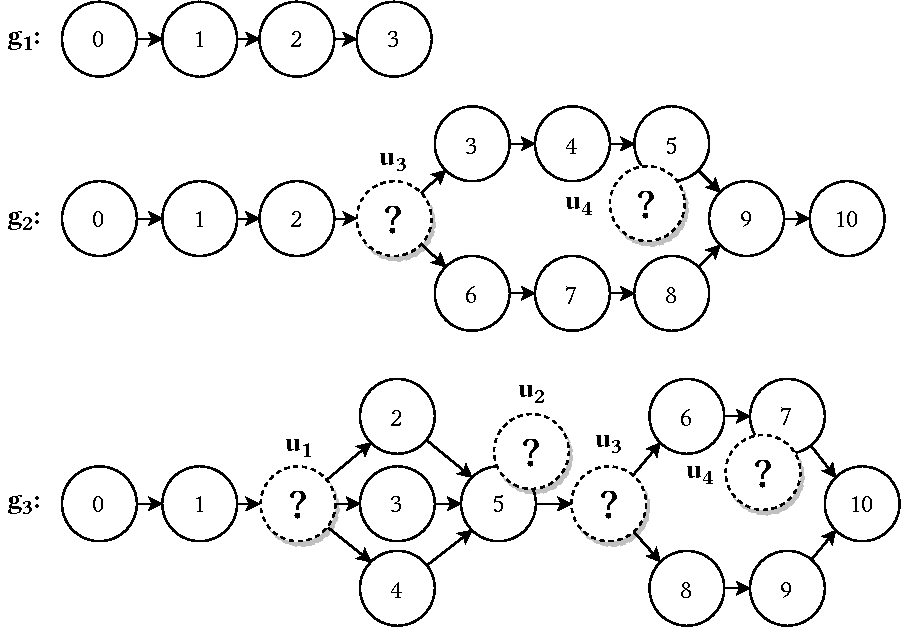
\includegraphics[width=\textwidth]{figures/chapter7/alltfgs.pdf}
    \caption{Simplified overview of all three \acfp*{TFG} of the running example with annotated primary and secondary uncertainties.}
    \label{fig:confidentialityanalysis:alltfgs}
\end{figure}

\autoref{fig:confidentialityanalysis:alltfgs} shows a simplified overview of all three \acp{TFG} of the running example.
We replace the vertices' names with numbers but keep the \emph{primary} uncertainty annotated to vertices, and \emph{secondary} uncertainty annotated to edges.
Note that we use a slightly different notation in this section to simplify the mathematical notation, e.g., $u_{1}$ refers to \U{1}.
This figure is based on \autoref{table:confidentialityanalysis:scenarios}, showing the scenarios of uncertainties \U{1} -- \U{4}, and \autoref{table:confidentialityanalysis:scenariostfgs}, showing the mapping of uncertainty sources to \acp{TFG}.
More detailed views of the second and third \acp{TFG} are shown in \autoref{fig:classification:dag} and \autoref{fig:confidentialityanalysis:dag}, respectively.
We also include the first \ac{TFG} representing the support contact request of the \emph{Customer}.
However, this \ac{TFG} is not affected by uncertainty, see \autoref{ch:runningexample}.

Let $G = \setted{g_{1}, g_{2}, \dots, g_{n}}$ where $n \geq 1$ be the nonempty finite set of all \acp{TFG} extracted from the architectural model, as introduced in \autoref{sec:confidentialityanalysis:framework}, and let $\abs{G}$ be its size.
In our running example, $G = \setted{g_{1},g_{2},g_{3}}$ and $\abs{G} = 3$.
Put simply, there are 3 extracted \acp{TFG}.
Let $U = \setted{u_{1}, u_{2}, \dots, u_{m}}$ where $m \geq 1$ be the nonempty finite set of all uncertainties, both \emph{primary} and \emph{secondary}, and let $ \abs{U}$ be the its size.
In our running example, $U = \setted{u_{1}, u_{2}, u_{3},u_{4}}$ and $\abs{U} = 4$.
Put simply, there are 4 uncertainties. 
We further split $U$ in $U_{P} \subseteq U$ to represent all \emph{primary} uncertainties and $U_{S} \subseteq U$ to represent all \emph{secondary} uncertainties in $U$.
This also means that $U = U_{P} \cup U_{S}$ and $U_{P} \cap U_{S} = \emptyset$.
In our running example, $U_{P} = \setted{u_{2}, u_{4}}$ and $U_{S} = \setted{u_{1}, u_{3}}$.
For each uncertainty source $u \in U $, let $ S_{u} = \setted{s_{u_{1}}, s_{u_{2}}, \dots, s_{u_{p}}}$ where $p \geq 1$ be the nonempty finite set of all uncertainty scenarios of $u$ and let $ \lvert S_{u} \rvert$ its size.
As discussed with \acp{NDFD} in \autoref{sec:confidentialityanalysis:typeagnostic}, $p \geq 1$ is trivially satisfied, as every uncertainty source has at least one default scenario.
In our running example, $ S_{u_{1}} = \{ s_{1}, s_{2}, s_{3} \}$ and $\abs{S_{u_{1}}} = 3$.
Put simply, the first uncertainty has three uncertainty scenarios, i.e., valid input, erroneous input, and malicious input, see \autoref{table:confidentialityanalysis:scenarios}.

Each uncertainty scenario brings variation into a \ac{TFG} and thus has to be analyzed separately.
This also applies to combinations of uncertainties, where every combination of all relevant scenarios of all relevant uncertainties has to be analyzed separately, i.e., the Cartesian product \cite{de_finetti_theory_2017}.
To minimize the analysis runtime and maximize its scalability, it is thus important to make a good estimation of what is \emph{relevant}.
Otherwise, the combination of scenarios can lead to the already discussed combinatorial explosion \cite{koziolek_automated_2011}.
We define $N$ as the number of \acp{TFG} that have to be analyzed in total.
In the following, we define three formulas to calculate this number, based on the underlying approach.
We define $N_{S}$ for the \emph{scenario-aware} analysis (\level{2}), $N_{G}$ for the \emph{graph-aware} analysis (\level{3}), and $N_{I}$ for the \emph{impact-aware} analysis (\level{4}).
Note that all three analysis approaches find the same confidentiality violations due to uncertainty, i.e., the accuracy is not affected.
However, the number of \acp{TFG} that have to be analyzed can differ.


The \emph{scenario-aware} analysis (\level{2}) does not consider \acp{TFG} but only combinations of scenarios.
Thus, for every possible scenario combination, every \ac{TFG} has to be analyzed which represents the least optimized approach.
We denote:

\begin{equation*}
N_{S} = \abs{G} \cdot \prod_{u \in U} \abs{S_{u}}
\end{equation*}

This is equivalent to generating all possible scenario combinations, applying them to all \acp{TFG}, and analyzing them, as introduced in \autoref{alg:confidentialityanalysis:scenarioaware}.
In our running example with 3 \acp{TFG} and 4 uncertainty sources, this means we have to analyze $N_{S} = \abs{G} \cdot \abs{S_{u_{1}}} \cdot \abs{S_{u_{2}}} \cdot \abs{S_{u_{3}}} \cdot \abs{S_{u_{4}}} = 3 \cdot 3 \cdot 4 \cdot 2 \cdot 2 = 144$ \acp{TFG}.
This is equivalent to analyzing all 3 \acp{TFG} in all 48 scenarios, as discussed in \autoref{sec:confidentialityanalysis:typespecifc}.


The \emph{graph-aware} analysis (\level{3}) does take \acp{TFG} into account and thus only has to consider combinations of scenarios in the same \ac{TFG}.
This is based on the finding that uncertainties in different flows, i.e., different \acp{TFG}, cannot affect each other, as discussed in \autoref{sec:impactanalysis:ufd}.
This highly reduces the amount of \acp{TFG} that have to be analyzed, especially in larger systems with many independent data flows.
To count the uncertainty sources $u \in U$ and its scenarios $S_{u}$ that impact a specific TFG $g \in G$, we define the \emph{impact function}:

\begin{equation*}
    f(g,u) = 
    \begin{cases}
        1,& \text{if there is no impact of } u \text{ on } g\\
        \abs{S_{u}},& \text{otherwise}
    \end{cases}
\end{equation*}

In our running example, $f(g_{2},u_{3}) = 2$, because the uncertainty $u_{3}$ in the \ac{TFG} $g_{2}$ has 2 scenarios.
To recall, the second \ac{TFG} represents the querying of items and Uncertainty \U{3} represents the deployment with the scenarios of being deployed on-premise or in the cloud.
$f(g_{1},u_{3}) = 1$, because the uncertainty $u_{3}$ has no effect on the first \ac{TFG}.
Put simply, this function yields the number of scenarios if the uncertainty is relevant for a \ac{TFG}; otherwise, it returns 1.
Using this function, we denote:

\begin{equation*}
    N_{G} = \sum_{g \in G} \prod_{u \in U} f(g,u)
\end{equation*}

This is equivalent to iterating over all \acp{TFG} and only generating the scenario combinations relevant for the current \ac{TFG}, as introduced in \autoref{alg:confidentialityanalysis:graphaware}.
In our example, the first \ac{TFG} has no uncertainty and $f$ always returns 1.
The second \ac{TFG} is only impacted by $u_{3}$ and $u_{4}$ while the third \ac{TFG} is impacted by all uncertainties.
In sum, this means: $N_{G} = (1 \cdot 1 \cdot 1 \cdot 1) + (1 \cdot 1 \cdot 2 \cdot 2) + (3 \cdot 4 \cdot 2 \cdot 2) = 1 + 4 + 48 = 53$ \acp{TFG}.
The number of \acp{TFG} that have to be analyzed by the \emph{graph-aware} approach is notably smaller compared to the \emph{scenario-aware} approach, i.e., $53 < 144$.
Although the third \ac{TFG} represents the worst case of combining all scenarios, the other \acp{TFG} are not affected.
Note that this formula only results in the same number as the \emph{scenario-aware} approach if all \acp{TFG} are affected by all uncertainties.
Trivially, this is the case if there is only one data flow within the system.
However, we assume that real-world software systems comprise more than a single data flow \cite{hahner_architecture-based_2023}.
Such a system would only provide a single functionality via a single interface with a single use case without any branching.
Thus, as \acp{TFG} are independent and an uncertainty impact can always assigned to a single \ac{TFG}, we find in general: 

\begin{equation*}
    N_{G} \leq N_{S}
\end{equation*}


The \emph{impact-aware} analysis (\level{4}) extends the \emph{graph-aware} analysis and additionally considers the transitive effect of the uncertainty scenarios.
By incrementally evaluating uncertainty scenarios, the impact of previous uncertainties in the same \ac{TFG} can be considered.
This enables us to analyze only those scenarios that are still relevant after other uncertainty scenarios have been applied in the direction of the data flow.
We consider uncertainty interactions between the \emph{secondary} uncertainties $U_{S}$ and \emph{primary} uncertainties $U_{P}$.
If an \emph{component} uncertainty, \emph{interface} uncertainty, or \emph{connector} uncertainty changes the edges of a \ac{TFG}, this affects all vertices---and all \emph{primary} uncertainties that affect such vertices---in the direction of the data flow, see \autoref{sec:confidentialityanalysis:typeagnostic}.

The easiest way to consider this in the calculation of relevant \acp{TFG} is to process all \acp{TFG} $g \in G$.
Similar to \autoref{alg:confidentialityanalysis:processvertex}, we replace all \emph{secondary} uncertainties $u \in U_{S}$ in all \acp{TFG} $g \in G$ with their scenarios.
Following the notion introduced in \autoref{sec:classification:dfd}, this means iterating over all $E_{u_{i}} \subseteq E$, i.e., all sets of alternative edges representing a \emph{secondary} uncertainty that form a subset of all edges of a \ac{DAG}.
For each edge $e \in E_{u_{i}}$, we create a copy of the current \ac{TFG} that contains the edge $e$ but none of the other edges in $E_{u_{i}}$.
The processing continues replacing \emph{secondary} uncertainty on the resulting \acp{TFG} until all \emph{secondary} uncertainties have been processed.
In sum, we define the function $p(G,U)$ that takes a set of \acp{TFG} $G$ and yields a set of \acp{TFG}, where all \emph{secondary} uncertainties in $U$ have been processed as described above.
As all uncertainties have at least one default scenario, we can say: $\abs{G} \leq \abs{p(G,U)}$.
Note that in contrast to \autoref{alg:confidentialityanalysis:processvertex}, we do not additionally process \emph{primary} uncertainty for the calculation as this uncertainty cannot alter edges in the \ac{TFG}.
Trivially, this means $\abs{p(G,U)} = \abs{p(G,U_{S})}$ and $\abs{G} = \abs{p(G,U_{P})}$.

In our running example, the second \ac{TFG} $g_{2}$ has one \emph{secondary} uncertainty $u_{3}$.
Applying this processing results in replacing the uncertainty $u_{3}$ with its affected edges, thereby creating 2 new \acp{TFG}, one with the edge $\flow{2}{3}$ and a second one with the edge $\flow{2}{6}$, see \autoref{fig:confidentialityanalysis:alltfgs}.
Thus, $\abs{p(\setted{g_{2}}, U)} = 2$.
The third \ac{TFG} $g_{3}$ has two \emph{secondary} uncertainties $u_{1}$ and $u_{3}$, with 3 and 2 scenarios, respectively.
Thus, $\abs{p(\setted{g_{3}}, U)} = 3 \cdot 2 = 6$.
We denote: 

\begin{equation*}
    N_{I} = \sum_{g \in p(G,U)} \prod_{u \in U_{P}} f(g,u)
\end{equation*}

This is equivalent to iterating over all vertices of all \acp{TFG} and taking the transitive impact of \emph{secondary} uncertainties into account, as introduced in \autoref{alg:confidentialityanalysis:impactaware}.
Note that we only calculate the product of \emph{primary} uncertainties, as we already considered the impact of the \emph{secondary} uncertainties in the processing $p(G,U)$.
In our running example, this does affect the calculation of the second and third \ac{TFG}.
As discussed previously, the second \ac{TFG} has one \emph{secondary} uncertainty.
After the processing of this uncertainty, only one of the two resulting \acp{TFG} is affected by the remaining \emph{primary} uncertainty.
This is the \ac{TFG} that represents the deployment in the cloud (\U{3}) that is affected by the provider's trustworthiness (\U{4}).
This effect becomes even bigger in the third \ac{TFG}.
Here, only half of the resulting \acp{TFG} represent a deployment in the cloud (\U{3}).
In sum, this means: $N_{I} = (1 \cdot 1) + ((1 \cdot 2) + (1 \cdot 1)) + ((4 \cdot 2) + (4 \cdot 2) + (4 \cdot 2) + (4 \cdot 1) + (4 \cdot 1) + (4 \cdot 1)) = 1 + (2 + 1) + (8 + 8 + 8 + 4 + 4 + 4) = 1 + 3 + 36 = 40$ \acp{TFG}.
We use parenthesis to highlight the \acp{TFG} after the processing.
This represents the minimum of scenarios and \acp{TFG} that have to be analyzed to identify all potential confidentiality violations, i.e., $40 < 53 < 144$.
As we replace every \emph{secondary} uncertainty in $U$ with additional graphs in $G$, we move them from the inner product to the outer sum in the formula.
Thus, we find in general: 

\begin{equation*}
    N_{I} \leq N_{G} \leq N_{S}
\end{equation*}





\section{Assumptions and Limitations}%
\label{sec:confidentialityanalysis:assumptions}

In this section, we discuss the assumptions and limitations of the different approaches of data flow analysis under uncertainty presented in this chapter.
This includes assumptions of single approaches and more general assumptions made in this chapter.
Note that we skip the limitations of the lower awareness levels \level{0} -- \level{3} compared to \emph{impact-aware} analysis (\level{4}) as we already comprehensively discussed their differences throughout this chapter.
The same applies to the comparison of \emph{type-specific} and \emph{type-agnostic} approaches.

\paragraph{Limitations of the data flow analysis framework}
Our approach for data flow analysis and the data flow analysis framework \cite{boltz_extensible_2024} are based on previous work in this field \cite{seifermann_architectural_2016,seifermann_identifying_2021,seifermann_unified_2021,seifermann_data-driven_2019,seifermann_detecting_2022,seifermann_architectural_2022,schneider_how_2024,schneider_microsecend_2023}.
Thus, we inherit some of the limitations.
First, the analysis operates on type-level, e.g., by analyzing usage scenarios and not individual users.
This restricts the expressiveness of analyzable confidentiality requirements \cite{seifermann_architectural_2022}.
Second, all four analysis approaches use the \ac{PCM} as an architectural model as previously discussed in \autoref{sec:impactanalysis:limitations}.
However, as the majority of the analysis is conducted on \acp{DFD}, the concepts should be generalizable.
First steps in this direction have already been taken \cite{boltz_extensible_2024}.
Third, the analysis does not respect state or time which limits the expressiveness but simplifies the analysis complexity \cite{seifermann_architectural_2022}.
Fourth, the labels used for confidentiality analysis represent discrete value sets, and there is no support for expressing continuous values other than mapping them to discrete values \cite{seifermann_architectural_2022}.
We refer to \textcite{seifermann_architectural_2022} for more detailed explanations of the reasoning behind these limitations.
Last, cycles within architectural models only have limited effects by only being traversed once.
However, there exist approaches for handling cycles in the construction of \acp{DAG} \cite{kramer_combining_1994,arp_analyzing_2024}.

\paragraph{Independence of data flow paths}
\textcite{seifermann_architectural_2022} discussed the assumption of independent data flow paths in data flow analysis.
Our data flow analysis framework presented in \autoref{sec:confidentialityanalysis:framework} follows this by assuming independence of extracted \acp{TFG} regarding the propagated labels that represent confidentiality-related characteristics of the software system.
Furthermore, we also assume that the impact of uncertainty in \acp{TFG} can be analyzed independently.
We argue that this assumption is reasonable.
The former can lead to an overestimation of confidentiality violations, which is acceptable.
The latter has been thoroughly discussed in \autoref{ch:classification} and \autoref{ch:impactanalysis}.

\paragraph{Modeling uncertainty scenarios}
The majority of approaches presented in this chapter are based on the assumption that modeling uncertainty scenarios is reasonable to express their effects on software systems, e.g., using design decision models \cite{koziolek_peropteryx_2011}, variation models \cite{walter_architecture-based_2023}, or uncertainty models \cite{hahner_model-based_2023}.
The description of uncertainty using scenarios has been discussed in the literature \cite{walker_defining_2003,mahdavi-hezavehi_classification_2017,armour_five_2000}, see \autoref{table:foundations:sources:locationlevel}.
\textcite{troya_uncertainty_2021} conducted a \acf{SLR} with 123 papers and support this assumption.
They found that \emph{design uncertainty} is usually expressed using uncertainty scenarios.

\paragraph{Analyzing unanticipated change}
We assume that the information required to model and analyze the software system under uncertainty is available to software architects.
A similar assumption has been made in the underlying approach for data flow analysis \cite{seifermann_architectural_2022} and also in earlier discussions of assumptions in \autoref{sec:classification:limitations} and \autoref{sec:impactanalysis:limitations}.
Similarly, we cannot express or analyze not yet identified uncertainty sources.
Nevertheless, we provide software architects with means to express uncertainty models within the architectural models and refine this model once more knowledge is gained.
The connection of data flow analysis to our catalog presented in \autoref{sec:classification:identification} further addresses this limitation. 

\paragraph{Multiple data flows and secondary uncertainty}
In this chapter, we present multiple approaches for data flow analysis under uncertainty.
The increased scalability of the \emph{graph-aware} analysis (\level{3}) and \emph{impact-aware} analysis (\level{4}) is based on two assumptions on the modeled software system.
First, we assume that real-world software systems comprise more than a single data flow path.
As discussed previously, such a system would only provide a single functionality via a single interface with a single use case without any branching.
Second, we assume the existence of \emph{secondary} uncertainty within the software system.
We argue that this is reasonable as three of the five uncertainty types introduced in \autoref{table:classification:classification:architecturalelementtype} represent \emph{secondary} uncertainty.
If this assumption does not hold, the latter analysis approaches are still applicable.
However, their benefits regarding the analysis complexity are decreased.

\paragraph{Limited support for uncertainty interactions}
Based on our findings on uncertainty propagation and \acp{UFD} presented in \autoref{sec:impactanalysis:ufd}, the \emph{impact-aware} analysis (\level{4}) supports simple uncertainty interactions.
However, this support is limited to the impact of \emph{secondary} uncertainty on \emph{primary} uncertainty.
Put simply, altering the edges of a \ac{DAG} can affect the flow of data to vertices and thus can also affect the impact of \emph{primary} uncertainty on these vertices.
Further uncertainty interactions can happen, e.g., between two \emph{primary} uncertainties where one uncertainty voids the impact of another uncertainty.
This limitation is similar to the overestimation of the uncertainty impact discussed in \autoref{sec:impactanalysis:limitations}.
Addressing this requires a higher expressiveness in the modeling and analysis as more fine-grained interactions between uncertainty and confidentiality have to be considered.

\paragraph{Mitigation of uncertainty}
We consider the automated mitigation of uncertainty as out of the scope of this thesis.
This includes the automated repair of uncertainty-afflicted software systems due to confidentiality violations.
Additionally, we only focus on finding all potential confidentiality violations due to uncertainty.
Analysis approaches that aim for fast feedback for software architects by returning partial results could thus further increase the analysis scalability.
We emphasize that advanced approaches to analysis, mitigation, and repair are expedient and that our analysis approaches can provide a comprehensive foundation for such endeavors. 

\paragraph{Uncertainty in confidentiality requirements}
We do not consider any uncertainty within confidentiality requirements that can occur, e.g., due to the relation to legal assessment \cite{boltz_model-based_2022}.
This would require means to express uncertainty-related variation not only as part of the software system but also in the specification of data flow constraints.
This could be achieved, e.g., by extending existing \acfp{DSL} \cite{hahner_modeling_2021,boltz_extensible_2024}.
Similar to the previous limitation, we emphasize the importance of this research but consider it to be out of scope for this thesis.





\section{Summary and Outlook}%
\label{sec:confidentialityanalysis:summary}

In this chapter, we presented multiple approaches to uncertainty-aware data flow analysis to identify potential confidentiality violations due to uncertainty.
This represents our third Contribution \C{3} and provides an answer to \RQ{3}.

First, we discussed the foundations required to define uncertainty-aware data flow analyses, as described with Problem \PR{3}{1}.
We presented an extensible framework for data flow analysis \cite{boltz_extensible_2024} that enables both black-box and white-box extensions \cite{taghavi_survey_2023,heinrich_composing_2021} of confidentiality analysis.
Here, we also introduced the concepts of \acp{TFG} and label propagation.
Afterward, we discussed which information is available in data flow analysis under uncertainty and how this information can be used.
To that end, we specified five levels (\level{0} -- \level{4}) of uncertainty awareness: The lack of uncertainty-awareness (\level{0}), naive approaches (\level{1}), scenarios-awareness (\level{2}), graph-awareness (\level{3}), and impact-awareness (\level{4}).
Uncertainty-aware data flow analyses that fall into one of these categories can be further categorized into type-specific and type-agnostic approaches.

Building on these foundations, we presented two \emph{type-specific} approaches to data flow analysis under uncertainty.
This addresses Problem \PR{3}{2}.
First, we introduced a \emph{scenario-aware} analysis (\level{2}) of structural uncertainty.
By combining the design space exploration approach PerOpteryx \cite{koziolek_peropteryx_2011,koziolek_automated_2011} with data flow analysis, we can identify confidentiality violations in software architecture candidates.
This enables the analysis of structural uncertainty, e.g., due to an uncertain deployment of a component.
Second, we introduced a \emph{graph-aware} analysis (\level{3}) of environmental uncertainty.
Here, we used fuzzy inference in the form of \acp{FIS} to express natural factors in the environment of a software system that can affect access control decisions and, thus, confidentiality.
We found that both analysis approaches share the representation of uncertainty sources as one or multiple scenarios.

Last, we moved towards \emph{type-agnostic} approaches for uncertainty-aware data flow analysis to address Problem \PR{3}{3}.
First, we presented a \emph{graph-aware} analysis (\level{3}) that uses variation modeling \cite{mehl_palladio_2022,walter_architecture-based_2023} to trace confidentiality violations back to uncertainty sources.
Being \emph{type-agnostic}, this approach supports all five uncertainty types introduced in \autoref{sec:classification:classification}.
To also support simple forms of uncertainty interactions, we introduced an \emph{impact-aware} analysis (\level{4}) thereafter.
We closed the gap between the uncertainty classification and confidentiality analysis by providing a meta model for modeling uncertainty sources and scenarios.
The analysis incrementally considers the impact of uncertainty within the data flow and thus can respect relations between multiple uncertainties.
We also introduced \abunai, our \ac{PCM}-based tooling for uncertainty \emph{impact-aware} data flow analysis (\level{4}).
We concluded this discussion by comparing the complexity of the presented analyses.

\RQ{3} asked about the analysis of confidentiality requirements using architecture-based data flow analysis that considers uncertainty within the architectural model and thus becomes uncertainty-aware.
To answer this question, we provided a discussion of available information, resulting awareness levels of data flow analyses and analysis complexity and scalability.
Furthermore, we presented four analysis approaches that differ in supported uncertainty types, awareness levels (\level{2} -- \level{4}) and type specificity.
As pointed out earlier, there is no single best answer to the question of architecture-based confidentiality analysis under uncertainty.
Thus, our approach to this chapter was to provide a comprehensive discussion of multiple solutions and their trade-offs.

There are multiple benefits of the variety of analysis approaches presented in this chapter with Contribution \C{3}.
In general, considering uncertainty within an analysis enables more precise and more comprehensive analysis results of a model and its context \cite{weyns_towards_2023,weyns_introduction_2020,perez-palacin_dealing_2014}.
Here, all four approaches can be used standalone, thus providing means to model and analyze different types of uncertainty.
An automated analysis like \abunai supports architects by reducing the manual effort, especially in large models with many independent data flows and many uncertainty sources \cite{hahner_model-based_2023}.
Furthermore, describing uncertainties as a first-class entity and part of the architectural model helps in the documentation \cite{hahner_classification_2023}.
Although we focused on confidentiality, our \emph{impact-aware} analysis is also an approach to consider uncertainty interactions within the architecture-based analysis.
Together with our finding on \acp{UFD}, this can be used to further address the \ac{UIP}.
Last, our data flow analysis framework can be used to define new analysis approaches, even without the need to focus on uncertainty \cite{boltz_extensible_2024}.

The contribution provided in this chapter was based on the findings from \readingpath{ch:classification} and \readingpath{ch:impactanalysis}.
We used many of the concepts introduced in these earlier chapters, e.g., the five uncertainty types, or the representation of uncertainty in \acp{DAG} as \emph{primary} and \emph{secondary} uncertainty.
Also, the foundations for uncertainty propagation and interaction were laid in these chapters.
The confidentiality analysis with respect to uncertainty represents the last step of the procedure presented in \readingpath{ch:overview}.
The next chapters show an overview of \readingpath{ch:evaluationscenarios} and then present the \readingpath{ch:evaluation} of all contributions.





\section{In Simpler Words}%
\label{sec:confidentialityanalysis:simple}

Confidentiality describes the property that information is not disclosed to persons or organizations that should not see this information.
Put simply, if you tell me a secret, I should keep it secret---treating it confidential.
The same applies to software systems and the data that is handled by these systems.
If you enter your personal data, such as your name, date of birth, or credit card details, into an online shop, you assume that you can trust the shop and that your information is treated confidentially.

Architecture-based confidentiality analyses have been proposed to analyze the confidentiality of a software system at a high abstraction or early in the system design.
These analyses use a model of the system and confidentiality requirements as input and identify confidentiality violations.
For example, if a law requires your confidential data to be stored on a server in the same country, but the system sends it across a border, this would represent a confidentiality violation.
To identify such violations, we analyze all data flows in a software architecture---this is called \emph{data flow analysis}.

In the previous chapters, we already introduced the notion of uncertainty and also discussed that uncertainty can negatively impact a software system's confidentiality.
For instance, if we do not know whether your data is actually sent to a server in another country, we cannot state that it is confidential.
To identify confidentiality violations under uncertainty, we define several uncertainty-aware data flow analyses.
In this chapter, we present four different analysis approaches that use different algorithms to see how uncertainty impacts confidentiality.
Some of these approaches are tailored to one uncertainty type, such as uncertainty in a software system's environment.
Other approaches support all uncertainty types that have been identified in \autoref{ch:classification}.
We call the former \emph{type-specific} analyses and the latter \emph{type-agnostic} analyses.
Additionally, we investigate the information used by the analysis and define five levels of uncertainty awareness.

Although the four presented approaches differ regarding the level of uncertainty awareness, they share the representation of uncertainty in the form of scenarios.
A scenario represents one possible outcome of uncertainty, e.g., whether your data flows across a country border.
The uncertainty-aware analysis considers these scenarios in analyzing confidentiality and returns only those scenarios that violate confidentiality.
This helps software architects to better assess whether or not an uncertainty is critical and should be mitigated.
Some approaches find such critical scenarios by checking all possible variations of the software architecture.
Other approaches use the available information in a more clever way and can exclude irrelevant scenarios early in the analysis.

The most advanced approaches center their analysis algorithm around uncertainty.
They treat uncertainty as a so-called first-class entity or first-class concern.
This means that uncertainty is of central importance and as important as every other element of the software architecture.
We find that considering uncertainty in this way helps to provide more and better information to the software architects.
Additionally, the analysis scales better for large software systems from the real world.
We also implemented such an analysis and provided it together with this thesis.
This represents the final contribution of this thesis and also concludes the procedure that has been introduced in \autoref{ch:overview}.
